%%
%%
\documentclass[preprint,3p,10pt,onecolumn,number,sort&compress]{elsarticle}
%\documentclass[final,3p,10pt,twocolumn,number,sort&compress]{elsarticle}

%% if you use PostScript figures in your article
%% use the graphics package for simple commands
%% \usepackage{graphics}
%% or use the graphicx package for more complicated commands
 \usepackage{graphicx}
 \usepackage{amsmath}
 \usepackage{stfloats}
 \usepackage{afterpage}
 \usepackage{placeins}
% \usepackage{xfrac}

%% or use the epsfig package if you prefer to use the old commands
%% \usepackage{epsfig}

%% The amssymb package provides various useful mathematical symbols
\usepackage{amssymb}
\usepackage{color}
%% The amsthm package provides extended theorem environments
%% \usepackage{amsthm}

%% The lineno packages adds line numbers. Start line numbering with
%% \begin{linenumbers}, end it with \end{linenumbers}. Or switch it on
%% for the whole article with \linenumbers after \end{frontmatter}.
%% \usepackage{lineno}

%\journal{Journal of Nuclear Materials}
\usepackage{lipsum}
\makeatletter
\def\ps@pprintTitle{%
 \let\@oddhead\@empty
 \let\@evenhead\@empty
 \def\@oddfoot{}%
 \let\@evenfoot\@oddfoot}
\makeatother
\begin{document}

\begin{frontmatter}

\title{\textit{Ab initio} molecular dynamics (AIMD) simulations of NaCl, UCl$_3$ and NaCl-UCl$_3$ molten salts}

\author[label1]{D. A. Andersson}
\ead{andersson@lanl.gov}
\author[label2,label3]{B. W. Beeler}
\address[label1]{Materials Science and Technology Division, Los Alamos National Laboratory P.O. Box 1663, Los Alamos, NM 87545, USA}
\address[label2]{Department of Nuclear Engineering, North Carolina State University, Raleigh, NC, United States}
\address[label3]{Idaho National Laboratory, Idaho Falls, ID 83415, United States}


\begin{abstract}
\textit{Ab initio} molecular dynamics (AIMD) simulations are used to calculate select thermophysical  
and thermodynamic 
properties of NaCl, UCl$_3$ and NaCl-UCl$_3$ molten salts. Following established approaches, the AIMD simulations  
include a model for Van der Waals interactions. The Langreth \& Lundqvist (vDW-DF2), DFT-D3, and density-dependent energy correction (DFT-dDsC) dispersion models are first tested for molten NaCl in order {\color{red}to} assess their accuracy for density and heat capacity predictions across a range of temperatures. 
Based on the NaCl results, the vdW-DF2 and DFT-dDsC methods are extended to the UCl$_3$ system and compared to available experimental data. 
Next, mixtures of NaCl-UCl$_3$ are investigated and analyzed with respect to the deviation from ideal solution behavior.  
For the DFT-dDsC simulations, density deviates by up to 2\% from an ideal mixture, with the maximum occurring close to the eutectic composition. 
The mixing energy also deviates from an ideal solution and exhibits a minimum of about -0.077 eV per formula unit, again close to the eutectic composition. Finally, the compressibility and species diffusivity of the pure and mixed salt systems are calculated. The diffusivities are slightly reduced in the mixed compared to the pure systems and the compressibilities loosely follow a linear correlation as a function of the UCl$_3$ composition.  
The trends observed for mixing properties are rationalized by correlating them to the coordination chemistry, which emphasizes the importance of maintaining the extended network formed by U and Cl ions as the NaCl concentration increases. The concentration at which breakdown of the extended network occurs, roughly coincides with the minimum of both the mixing energy and the deviation from ideal solution behavior for density.
\end{abstract}

%\begin{keyword}
%% keywords here, in the form: keyword \sep keyword

%% MSC codes here, in the form: \MSC code \sep code
%% or \MSC[2008] code \sep code (2000 is the default)

%\end{keyword}

\end{frontmatter}

%%
%% Start line numbering here if you want
%%
% \linenumbers

%% main text
\section{Introduction}
\label{sec:intro}
Molten salt reactors (MSRs) are among the advanced concepts pursued under the Generation IV nuclear energy technology umbrella. However, the basic concept is not new and was first developed as part of the effort to power aircrafts with nuclear energy in the 1950's~\cite{Rosenthal}. Later in the 1960's, Oak Ridge National Laboratory (ORNL) built and operated the Molten-Salt Reactor Experiment (MSRE)~\cite{MSRE1,MSRE2}. This reactor used a fluoride salt with uranium as fuel. Fluoride salts are still highly relevant and proposed in several designs. In addition, chloride salts are being considered for MSRs operating in the fast neutron spectrum. The present study focuses on chloride salts, in particular the NaCl-UCl$_3$ system, which is one of the primary fuel salt candidates.

Experimental characterization of UCl$_3$ densities have been reported by Janz et al.~\cite{Janz1988}, Desyatnik et al.~\cite{Desyatnik}, and most recently by Parker et al.~\cite{Parker}. The density correlation derived from the first experimental data set deviates significantly from Desyatnik et al.~\cite{Desyatnik} and Parker et al. ~\cite{Parker}. The latter two are considered to be the most accurate data.
Desyatnik et al.~\cite{Desyatnik} also investigated the density of NaCl-UCl$_3$ mixtures. They identified a negative deviation from an ideal solution across most of the composition range, with the high-temperature UCl$_3$-rich region deviating slightly from this trend. Parker et al. ~\cite{Parker} measured the density of the mixed systems in the NaCl-rich region using neutron radiography and reported correlations for the density as function of temperature at select compositions. The data points calculated from the correlations are scattered around the density expected for an ideal mixture, perhaps, with a trend towards a small positive deviation from an ideal solution, though the magnitude seems to be within the specified uncertainty of the correlation. 
Maatsura et al.~\cite{Matsuura} measured the mixing energies of NaCl-UCl$_3$ at 1173 K, which highlighted a negative deviation from ideal solution behavior (exothermic reaction) with a minimum of $-0.07$ to $-0.08$ eV per formula unit close to the eutectic composition ($x\approx 0.35$, where $x$ is the UCl$_3$ fraction), but perhaps slightly shifted towards the 50-50 composition. There are two Calphad assessments of the NaCl-UCl$_3$ system~\cite{BENES2008, YIN2020}. The magnitude and shape of the NaCl-UCl$_3$ mixing energies are noticeably different between the two assessments~\cite{YIN2020}. The assessment by Benes et al.~\cite{BENES2008} arrived at a form with a minimum close to the eutectic composition, while Yin et al.~\cite{YIN2020} used the experimental data due to Matsuura et al.~\cite{Matsuura} as input, which resulted in a more negative mixing energy that is shifted slightly closer to the 50-50 composition. The magnitude of the mixing energy is off by about 50\% between the two assessments. The experimental data on density and mixing energies will be further discussed in Sec. \ref{sec:results}.

The sparse and sometimes contradictory experimental data on molten salts in general, and the NaCl-UCl$_3$ system in particular, provides justification for pursuing modeling and simulation as a complementary approach to gain improved understanding. This opportunity is already acknowledged in the literature. Both classical molecular dynamics (CMD) and \textit{ab initio} molecular dynamics (AIMD) simulations have been used to study chloride salts involving actinides~\cite{Li,Li2020,Nam2015,SONG,VANOUDENAREN2021117470} and the related NaCl base salt~\cite{NGUYEN2021115262,LI2021100359,Tovey}. Li et al.~\cite{Li} used AIMD simulations to study the local structure of UCl$_3$, UCl$_4$, and mixtures of UCl$_3$, UCl$_4$ and NaCl at 1173 K. This study showed good agreement with experiments for the radial distribution function of the first coordination shell and identified network formation of UCl$_3$ units in mixed NaCl-UCl$_3$ salts~\cite{Li}.  
In order to study temperature-dependent thermophysical properties, a semi-empirical potential based on the polarizable ion model was developed~\cite{Li2020}. This potential successfully predicted density, thermal conductivity, and viscosity, though validation is challenged by the lack of experimental data. van Oudenaren et al.~\cite{VANOUDENAREN2021117470} used the same polarizable ion model to calculate additional properties, such as density, heat capacity and mixing energies as function of temperature and compared the results to available experimental data and the thermodynamic models referenced in the previous paragraph. 
Nam et al.~\cite{Nam2015} studied the solution thermodynamics of dilute concentrations of UCl$_3$ in a base salt and investigated the properties of base salts for different Van der Waals interaction models. Song et al.~\cite{SONG} performed AIMD simulations of densities and transport properties in a LiCl-KCl eutectic salt with a small concentration of UCl$_3$. 

In the present study, AIMD simulations relying on different models for the Van der Waals interactions were used to predict temperature-dependent thermophysical (density, compressibility, and diffusivity) and thermodynamic (mixing energy and heat capacity) properties of NaCl, UCl$_3$, and NaCl-UCl$_3$. The standard PBE exchange-correlation potentials typically used were extended to include a Hubbard $U$ model for the actinide 5f electrons. This extension has not previously been utilized for studying actinide salts. The purpose of the study was first to determine with what accuracy fundamental properties can be predicted by AIMD simulations for actinide containing salts, second to populate some of the data gaps that exist in the literature, and third to provide understanding of the link between coordination chemistry and properties. 

This paper is organized as follows. The methodology is described in Sec. \ref{sec:method}, followed by results and discussion in Sec. \ref{sec:results}. First, the benchmark for NaCl is presented, after which the UCl$_3$ results are reviewed followed by NaCl-UCl$_3$ mixtures. The implications of the results are discussed in Sec. \ref{sec:discussion} and, finally, conclusions are presented in Sec. \ref{sec:conclusions}. 

\section{Methodology}
\label{sec:method}
{\color{red}\subsection{Density functional theory}}
The AIMD simulations were performed with the VASP code~\cite{Kresse1996}. All simulations used the $\Gamma$ point for integration in reciprocal space. The accurate simulation setting was utilized in VASP, but the plane wave cut-off energy was increased above the standard setting to 400 eV. Gaussian smearing with a smearing parameter of 0.05 eV was used for the partial occupancies of the wave functions. The convergence criteria for the electronic minimization was at most 10$^{-3}$ eV for NaCl and $5\times10^{-3}$ eV for salts containing uranium. The Projector Augmented Wave (PAW) method was used to describe the core electrons~\cite{PAW1,PAW2}. The PAW potentials supplied with VASP for the PBE exchange-correlation potential were utilized, unless otherwise noted. For Na, the pseudopotential version that only includes the \textit{s} electron(s) in the valence shell {\color{red}(3s$^{1}$)} was used with the dDsC and DFT-D3 methodology, while the version that also includes the semi-core \textit{p} electrons {\color{red}(2p$^6$3s$^{1}$)} was utilized for the vdW-DF2 simulations. Although different choices were made for the simulations with regards to the Na potential, the results are not sensitive to this choice at a scale that impacts the conclusions of the present study. The PAW potential for Cl also included \textit{p} electrons {\color{red}(3s$^2$3p$^5$)} and for U it included the outer \textit{s}, \textit{p}, {\color{red}\textit{p}} and \textit{f} electrons {\color{red}(6s$^2$6p$^6$5f$^3$6d$^1$7s$^2$)} in the valance shell. 

%\subsection{Supercell Size}
{\color{red}The simulations used a range of supercell sizes with the largest consisting of 216 (NaCl), 216 (UCl$_3$) and 134-184 (NaCl-UCl$_3$ mixtures) atoms. The smallest cells for the same systems contain 64, 64 and 60-72 atoms, respectively.  {\color{red} The rationale for these cell sizes are provided in Sec. \ref{sec:size}.
For NaCl and UCl$_3$ the supercells were created by one of two methods. In the first method, the crystalline unit cell is replicated to generate a supercell, followed by melting of the lattice by performing high temperature MD simulations. The mixed supercells were created by replacing Na ions with U ions or vice versa, in some cases additional molecular units were added to ensure that a suitable number of atoms were maintained in the supercells. In the second method, the PACKMOL package \cite{packmol} was utilized to randomly insert individual molecules of NaCl and UCl$_3$ in the targeted concentration, followed by high temperature equilibration.
%\subsection{Application of the Hubbard U term}

The generalized gradient approximation (GGA) can fail to describe systems with localized (strongly correlated) \textit{f} electrons. This is often remedied by applying a Hubbard-like term to treat the strong on-site Coulomb interaction, commonly referred to as DFT+$U$ (also LDA+$U$ or GGA+$U$) \cite{rohrbach2003}. The appropriate magnitude of the applied screening needs to be uniquely determined for each element within each compound. {Based on results \color{red} in Sec. \ref{sec:hubbard}, it was determined that a U$_{eff}$ value of 4 eV (in the case of Dudarev) or a $U$ value of 4.5 eV and a J value of 0.51 eV (in the case of Lichtenstein) should be utilized for the NaCl-UCl$_3$ system. {\color{red}These settings were used for all systems, except where explicitly stated otherwise.} Differences between the two implementations of the Hubbard $U$ term should be statistically insignificant.}}

%The rotationally invariant approach of Dudarev \cite{dudarev1998} was implemented to investigate the effects of Coulombic screening, with the vdW-DF2 Van der Waals functional. The density, bandgap, and energy per molecule were analyzed as a function of U-J (U$_{eff}$) in increments of 1 eV for both UCl$_3$ and NaCl-33UCl$_3$ at 1250 K, in the ferromagnetic (FM) and anti-ferromagnetic (AFM) states. It should be emphasized that the Hubbard $U$ term was only applied to the \textit{f} electrons of uranium. 

%The zero-pressure density was determined by constructing pressure as a function of volume curves as a function of U$_{eff}$ at 1250 K for both the FM and AFM states. As will be discussed later, there is not an exact correspondence between the AIMD predicted densities and the experimental densities, but reasonable agreement is achieved. There exists a general trend of decreasing density with increasing U$_{eff}$, and that the AFM state predicts a slightly higher density (lower volume) than the FM state. These zero-pressure volumes are then utilized to determine the electronic density of states and the energy per molecule of their respective systems. A full discussion of densities is included in Sec. \ref{sec:results}. 

%The electronic density of states of AFM UCl$_3$ with a U$_{eff}$ of 0 and 4 eV is shown in Figure \ref{fig:DOS}a. It can be seen that at a U$_{eff}$ of 0 eV with no Coulombic screening, UCl$_3$ is electronically a conductor. It is known that this molten salt exhibits insulating properties with at least a minimal band gap. With the application of the Hubbard $U$ term, an insulating electronic structure is induced, as can be seen in Figure \ref{fig:DOS}b. The magnitude of the bandgap changes as a function of the magnitude of $U_{eff}$, with no bandgap below 2 eV, and the bandgap progressively increasing up to approximately 2.3 eV for a $U_{eff}$ of 5 eV. The magnitude of the bandgap of UCl$_3$ has not been experimentally determined, removing the possibility of fitting the U$_{eff}$ to the experimental bandgap. 

%It was also observed that the preferred magnetic state changes as a function of U$_{eff}$, with FM being preferred in the low U$_{eff}$/conducting region, and the AFM state preferred in the high U$_{eff}$/insulating region. This was identified by analyzing the energy per formula unit as a function of Hubbard $U$ magnitude. It is presumed that at high temperatures there would not be an ordered series of spins, and that is confirmed within this work, given that the electronic structure is appropriately accounted for. A previous study \cite{Li} investigated UCl$_3$ in the FM state without DFT+$U$ corrections. Although it was shown above that this incorrectly produces an electronically conductive molecular system, the choice of the FM state, given the absence of a Hubbard $U$ term, is not wholly incorrect. For a U$_{eff}$ value of 0, the FM state is the energetically preferred form of magnetism. 

%It is clear that a value of U$_{eff}$ greater than 2 eV is required to ensure the proper insulating electronic structure, and that this system prefers an AFM state. However, the actual magnitude of the optimal U$_{eff}$ value remains unknown. Thus, a further analysis on NaCl-33UCl$_3$ was performed to observe what trends in the electronic structure and energy per molecule exist as a function of U$_{eff}$. It was observed that at a U$_{eff}$ value of greater than 1 eV, an insulating electronic structure was induced, while the absence of the Hubbard $U$ term yielded a conducting system. Additionally, the AFM state becomes energetically favorable above a U$_{eff}$ of 2 eV. The trends in the density for NaCl-33UCl$_3$ as a function of U$_{eff}$ are statistically indistinguishable from those for UCl$_3$. This investigation served to reinforce the findings that value of U$_{eff}$ greater than 2 eV is required to ensure the proper insulating electronic structure, and that the NaCl-UCl$_3$ system prefers an AFM state. 

%Finally, the constrained DFT linear-response method \cite{PhysRevB.71.035105} was utilized within the Lichtenstein approach \cite{PhysRevB.52.R5467} for the Hubbard $U$ term of UCl$_3$. An approximate $U$ value range of 3.0-4.5 eV was determined and the J value was set to 0.51 eV. These values are similar to those proposed for UO$_2$ \cite{dudarev}. Given the lack of high-fidelity experimental data to serve as a basis for optimization of the Hubbard $U$ magnitude, it was determined that a U$_{eff}$ value of 4 eV (in the case of Dudarev) or a $U$ value of 4.5 eV and a J value of 0.51 eV (in the case of Lichtenstein) should be utilized for the NaCl-UCl$_3$ system. Differences between the two implementations of the Hubbard $U$ term should be statistically insignificant.

%\begin{figure*}[h]
%\centering
%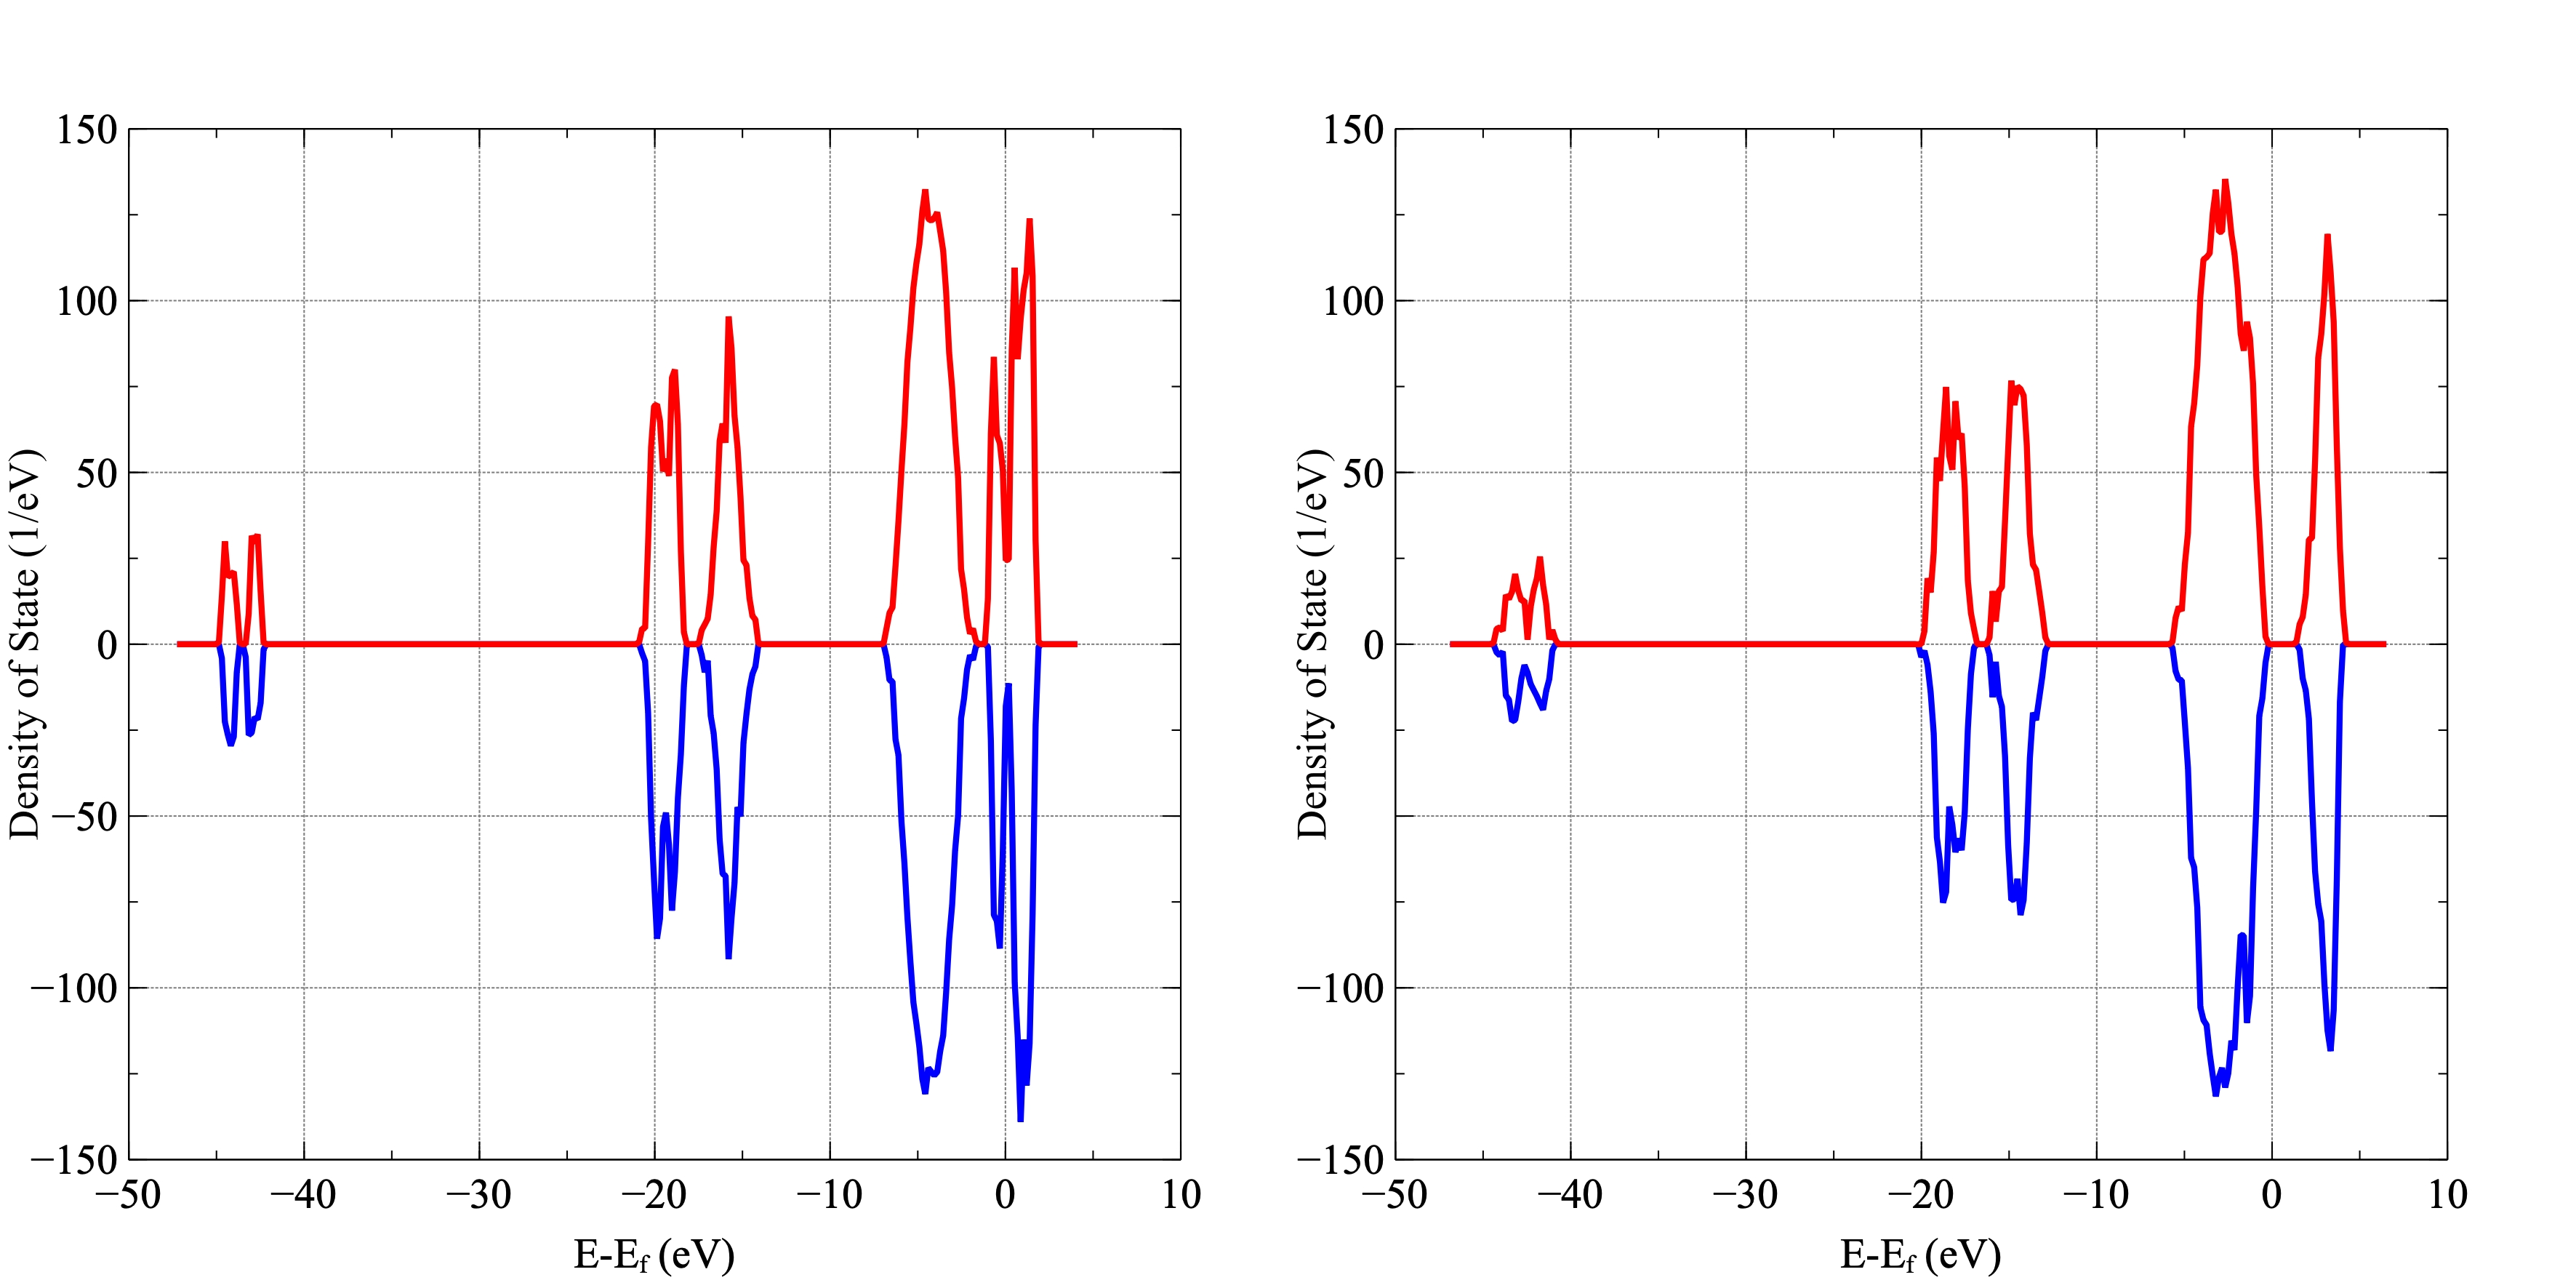
\includegraphics[width=0.9\textwidth]{fig3.jpg}
%\caption{The predicted density of states for simulations of AFM molten UCl$_3$ at 1250 K, a) not including a Hubbard $U$ model, and b) a Hubbard U value of 4 eV.} 
%\label{fig:DOS}
%\end{figure*}

%%\FloatBarrier

%\subsection{Van der Waals Dispersion}

It is well-established in the literature that Van der Waals, or dispersion, interactions are critical for reproducing the density of molten salts by DFT methods~\cite{Li,Nam2014,Nam2015}. In general, density functional theory methods are unable to describe Van der Waals dispersion (vdW) forces. A pragmatic method to work around this problem is to add a correction to the conventional Kohn-Sham DFT energy. This is performed through the addition of a vdW correction, or a replacement of the exchange-correlation functional to account for dispersion interactions. Given that there are numerous implementations of dispersion interaction, the choice of which dispersion interaction to utilize can be material and system dependent, and unknown without prior testing. Previous simulations have used both the DFT-D3~\cite{Li,Grimme} and the Langreth \& Lundqvist (vdW-DF2)~\cite{Nam2015,Dion,Klimes} methodologies for various molten chloride salts. Both methods were used in the present study. In addition, the density-dependent energy correction (DFT-dDsC) method~\cite{Steinmann2011,Steinmann2} was used with the goal of improving accuracy. The DFT-dDsC method does not include parameters for \textit{f} elements in the standard VASP version. In order to enable simulations the corresponding parameters were taken from Refs. ~\cite{Kim} ($C_6=4.889$ au and $r_0=6.416$ au) and~\cite{pol} ($\alpha=129.0$ au).} 

\subsection{AIMD simulations}
The AIMD simulations for the molten salt supercells were performed using isobaric (NPT) conditions unless otherwise noted. The primary intent of the NPT simulations (with the pressure set to zero) is to evaluate density, thermal expansion, heat capacity, and mixing energy. All NPT ensemble simulations used the the Langevin thermostat in VASP. For the NPT simulations, the temperature friction coefficient was set to 10 ps$^{-1}$ and the friction coefficient for the lattice degrees of freedom to 1 ps$^{-1}$. The time step was set to 2 fs for production runs between 1000 K and 1500 K. Around and below 1000 K, a larger time step of up to 5 fs is warranted due to the slow dynamics of uranium ions.

Pre-equilibrium and equilibration simulations were performed that involved melting the lattice and ensuring convergence of the total energy and pair distribution function for the temperature of interest. After pre-equilibration and equilibration, production simulations follow for, in most cases, at least 20 ps, though for a few limited cases simulation times were reduced to between 10 and 15 ps due to difficulties obtaining and then maintaining a well converged solution or because of the scoping nature of DFT-D3 simulations for NaCl. Some cases used longer production simulations, in particular this applies to the simulations based on smaller supercells and systems containing a mixture of UCl$_3$ and NaCl (up to 75 ps). NPT simulations require long equilibration times and may sometimes leave the equilibrium state due to distortions of the supercell, which is in part a consequence of applying the technique to somewhat small supercells. All simulations were inspected to avoid sampling such regimes. Additionally, an NVT ensemble was applied to obtain compressibilities, densities, heat capacities, and diffusivities. Only the vdW-DF2 dispersion functional was utilized for NVT ensembles. 

Properties were calculated by averaging over the production simulation (not including the equilibration or pre-production time). Densities were trivially obtained from the supercell volume and heat capacities from the slope of the total internal energy ($E_{tot}$) as function of temperature. 
\begin{equation}
\label{eq:cp}
C=\frac{\partial E_{tot}}{\partial T}
\end{equation}
This corresponds to heat capacity at constant pressure ($C_p$). Mixing energies were calculated from the potential energy ($E_{pot}$) of the mixed salt with pure NaCl and UCl$_3$ at the same temperature as the reference. 
\begin{equation}
\begin{split}
E_{mix}=E_{pot}(U_xNa_yCl_{3x+y})-xE_{pot}(UCl_3)-yE_{pot}(NaCl)
\end{split}
\end{equation}

The compressibility is calculated as the negative of the inverse equilibrium volume multiplied by the derivative of the volume as a function of pressure, as in Eq. \ref{eq:compress}. The volume as a function of pressure is determined by sampling multiple volumes in an NVT ensemble, and calculating the time-averaged pressure. 

\begin{equation}
\label{eq:compress}
\beta = -\frac{1}{V} {\left(\frac{dV}{dp}\right)}
\end{equation}

Diffusivities were calculated by tracking the mean-squared displacement (MSD) over three unique 20 ps simulations in an NVT ensemble. The MSD was verified to follow a linear trend as a function of time, and the first 4 ps were removed to determine the dependence of the MSD with time. The total, Na, Cl, and U diffusivities were determined via Einstein's equation:
\begin{equation}
MSD(t)=\sum_i^N (\mathbf{r^i(t)} - \mathbf{r^i(0)})^2 = N\times6Dt,
\end{equation}
where $i$ denotes an ion, $N$ is the total number of ions, $\mathbf{r^i}$ is the position vector, $D$ is the diffusivity, and $t$ is time. In the case of the total diffusivity, the diffusion coefficients are determined on a per formula unit basis, instead of on a per-atom basis. 

\section{Results}
\label{sec:results}

{\color{red}\subsection{Supercell Size}
\label{sec:size}
The differently sized supercells were investigated in order to understand and optimize the compromise between computational efficiency, enabling sampling in the time domain, and accuracy with respect to long range interactions. The radial distribution function (RDF) was used as the most basic measure of the adequacy of the supercell size, with convergence with respect to the targeted thermophysical and thermodynamic properties following suit. All the supercells investigated properly capture the expected radial distribution function in the liquid state. This behavior is exemplified in Figures \ref{fig:radial}a) and \ref{fig:radial}b) for UCl$_3$ and NaCl supercells of different size, respectively. The smaller cells predict essentially identical radial distribution functions across the full range for NaCl and up to 9~\AA{} for UCl$_3$, with small differences above that range for the U-U correlation, as compared to the larger cells, and enable improved computational efficiency. Although the larger cells may still be more accurate for, e.g., mixed salts exhibiting complex radial distribution functions, the situation is further complicated by the need to sample sufficient configurations to resolve the preferred short and intermediate range distribution of ionic species in network forming salts such as those containing UCl$_3$~\cite{Li}. This requires fairly long simulation times. Proper sampling is easier to achieve in smaller supercells given the computational cost of AIMD simulations, even though the radial distribution function itself, as well as other properties, may be better described in a larger supercell. For this reason, the results in Sec. \ref{sec:results} tend to use supercells of small size. Figure \ref{fig:NaClsize} compares the results of the NaCl density and energy, related to the heat capacity, as function of temperature for the small and large cells. Given the good agreement between the results from different supercells, density and heat capacity are considered accurately represented by all supercell sizes that were investigated. A similar result confirming the accuracy of the smaller cell was obtained for UCl$_3$. 
The small variations between supercells in Figure \ref{fig:NaClsize} are more likely related to sampling differences, rather than due to the supercell size. 

\begin{figure*}[htb]
\centering
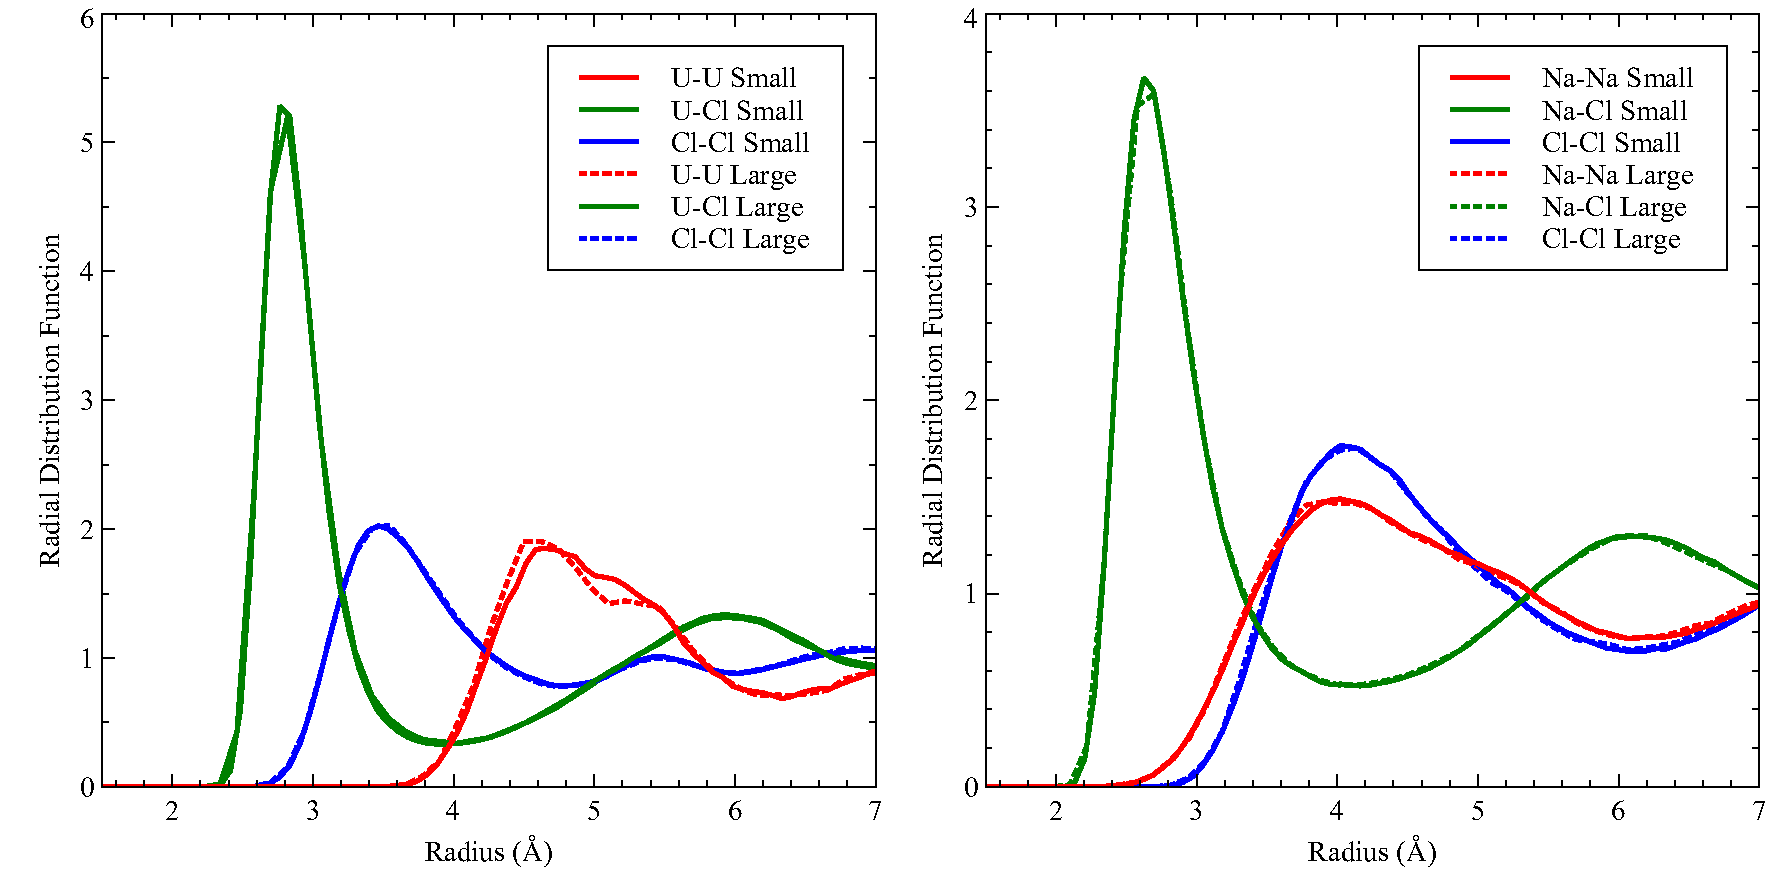
\includegraphics[width=0.9\textwidth]{fig1.pdf}
\caption{The predicted radial distribution function in a) UCl$_3$ and b) NaCl obtained by supercells containing 64 (small) and 216 (large) atoms at 1250 K.} 
\label{fig:radial}
\end{figure*}

\begin{figure*}[htb]
\centering
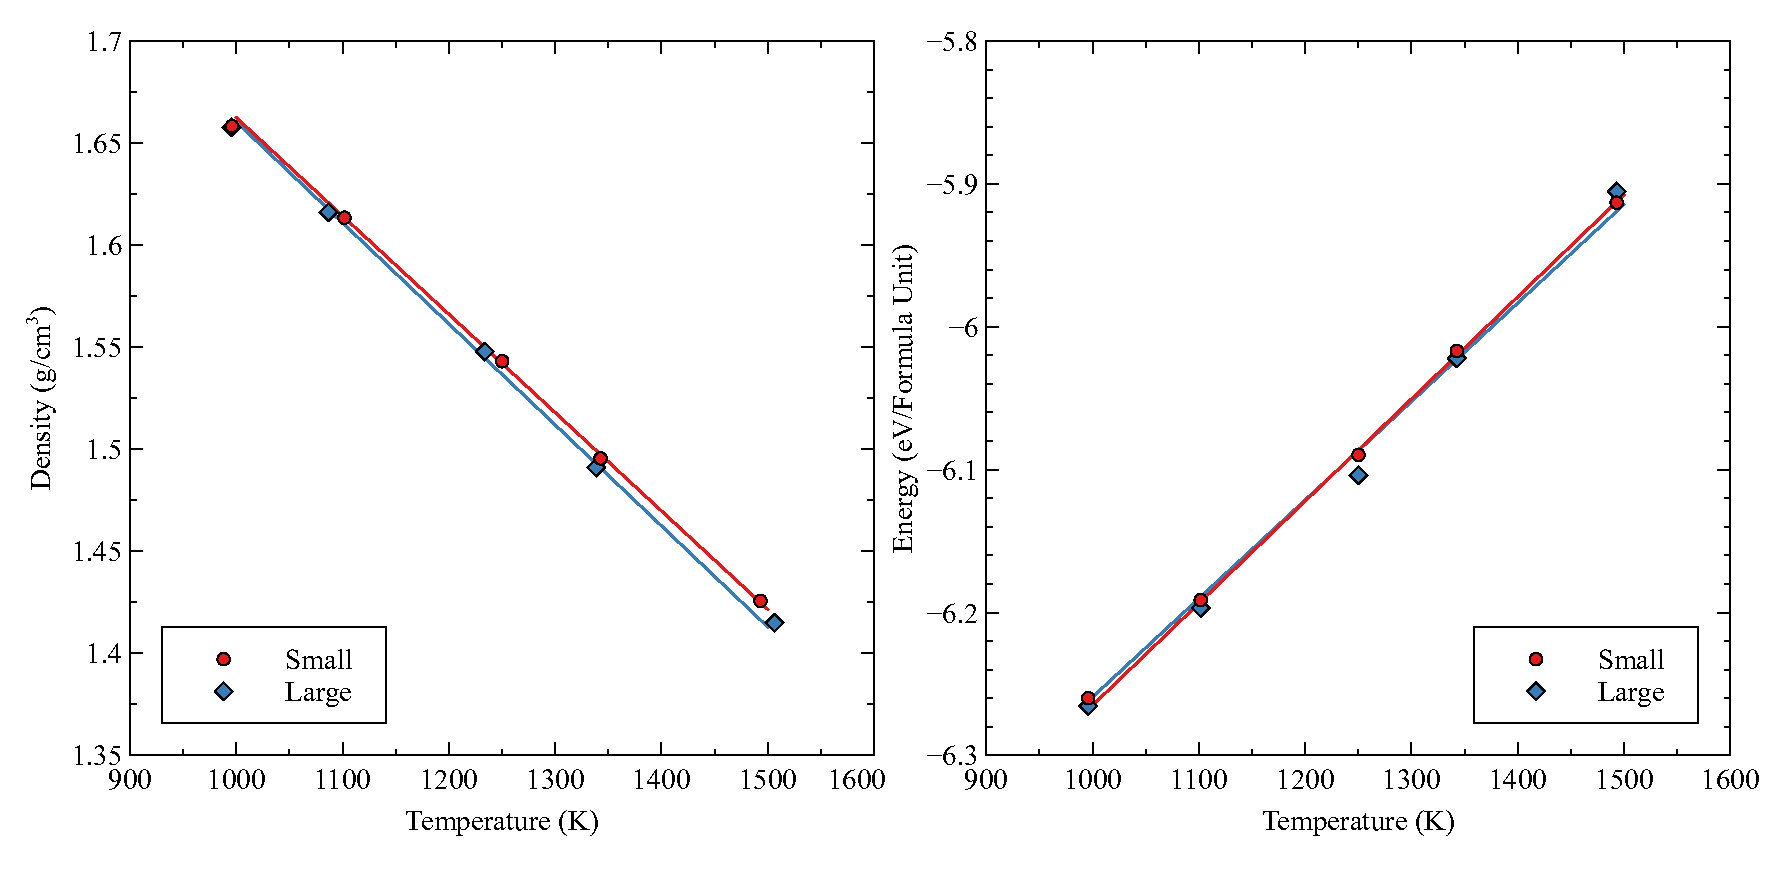
\includegraphics[width=0.9\textwidth]{fig2.pdf}
\caption{a) Calculated density and b) total energy of NaCl as function of temperature for the large and small supercells. The lines are least-squares fits to data points and the slope represents the heat capacity.} 
\label{fig:NaClsize}
\end{figure*}
}

{\color{red}\subsection{Application of the Hubbard U term}
\label{sec:hubbard}
%The generalized gradient approximation (GGA) can fail to describe systems with localized (strongly correlated) \textit{f} electrons. This is often remedied by applying a Hubbard-like term to treat the strong on-site Coulomb interaction, commonly referred to as DFT+$U$ (also LDA+$U$ or GGA+$U$) \cite{rohrbach2003}. The appropriate magnitude of the applied screening needs to be uniquely determined for each element within each compound. {Based on results \color{red} in Sec. \ref{sec:hubbard}, it was determined that a U$_{eff}$ value of 4 eV (in the case of Dudarev) or a $U$ value of 4.5 eV and a J value of 0.51 eV (in the case of Lichtenstein) should be utilized for the NaCl-UCl$_3$ system. Differences between the two implementations of the Hubbard $U$ term should be statistically insignificant.}
The rotationally invariant approach of Dudarev \cite{dudarev1998} was implemented to investigate the effects of Coulombic screening, with the vdW-DF2 Van der Waals functional. The density, bandgap, and energy per molecule were analyzed as a function of U-J (U$_{eff}$) in increments of 1 eV for both UCl$_3$ and NaCl-33UCl$_3$ at 1250 K, in the ferromagnetic (FM) and anti-ferromagnetic (AFM) states. It should be emphasized that the Hubbard $U$ term was only applied to the \textit{f} electrons of uranium. 

The zero-pressure density was determined by constructing pressure as a function of volume curves as a function of U$_{eff}$ at 1250 K for both the FM and AFM states. As will be discussed later, there is not an exact correspondence between the AIMD predicted densities and the experimental densities, but reasonable agreement is achieved. There exists a general trend of decreasing density with increasing U$_{eff}$, and that the AFM state predicts a slightly higher density (lower volume) than the FM state. These zero-pressure volumes are then utilized to determine the electronic density of states and the energy per molecule of their respective systems. A full discussion of densities is included in Sec. \ref{sec:results}. 

The electronic density of states of AFM UCl$_3$ with a U$_{eff}$ of 0 and 4 eV is shown in Figure \ref{fig:DOS}a. It can be seen that at a U$_{eff}$ of 0 eV with no Coulombic screening, UCl$_3$ is electronically a conductor. It is known that this molten salt exhibits insulating properties with at least a minimal band gap. With the application of the Hubbard $U$ term, an insulating electronic structure is induced, as can be seen in Figure \ref{fig:DOS}b. The magnitude of the bandgap changes as a function of the magnitude of $U_{eff}$, with no bandgap below 2 eV, and the bandgap progressively increasing up to approximately 2.3 eV for a $U_{eff}$ of 5 eV. The magnitude of the bandgap of UCl$_3$ has not been experimentally determined, removing the possibility of fitting the U$_{eff}$ to the experimental bandgap. 

It was also observed that the preferred magnetic state changes as a function of U$_{eff}$, with FM being preferred in the low U$_{eff}$/conducting region, and the AFM state preferred in the high U$_{eff}$/insulating region. This was identified by analyzing the energy per formula unit as a function of Hubbard $U$ magnitude. It is presumed that at high temperatures there would not be an ordered series of spins, and that is confirmed within this work, given that the electronic structure is appropriately accounted for. A previous study \cite{Li} investigated UCl$_3$ in the FM state without DFT+$U$ corrections. Although it was shown above that this incorrectly produces an electronically conductive molecular system, the choice of the FM state, given the absence of a Hubbard $U$ term, is not wholly incorrect. For a U$_{eff}$ value of 0, the FM state is the energetically preferred form of magnetism. 

It is clear that a value of U$_{eff}$ greater than 2 eV is required to ensure the proper insulating electronic structure, and that this system prefers an AFM state. However, the actual magnitude of the optimal U$_{eff}$ value remains unknown. Thus, a further analysis on NaCl-33UCl$_3$ was performed to observe what trends in the electronic structure and energy per molecule exist as a function of U$_{eff}$. It was observed that at a U$_{eff}$ value of greater than 1 eV, an insulating electronic structure was induced, while the absence of the Hubbard $U$ term yielded a conducting system. Additionally, the AFM state becomes energetically favorable above a U$_{eff}$ of 2 eV. The trends in the density for NaCl-33UCl$_3$ as a function of U$_{eff}$ are statistically indistinguishable from those for UCl$_3$. This investigation served to reinforce the findings that value of U$_{eff}$ greater than 2 eV is required to ensure the proper insulating electronic structure, and that the NaCl-UCl$_3$ system prefers an AFM state. 

Finally, the constrained DFT linear-response method \cite{PhysRevB.71.035105} was utilized within the Lichtenstein approach \cite{PhysRevB.52.R5467} for the Hubbard $U$ term of UCl$_3$. An approximate $U$ value range of 3.0-4.5 eV was determined and the J value was set to 0.51 eV. These values are similar to those proposed for UO$_2$ \cite{dudarev}. Given the lack of high-fidelity experimental data to serve as a basis for optimization of the Hubbard $U$ magnitude, it was determined that a U$_{eff}$ value of 4 eV (in the case of Dudarev) or a $U$ value of 4.5 eV and a J value of 0.51 eV (in the case of Lichtenstein) should be utilized for the NaCl-UCl$_3$ system. Differences between the two implementations of the Hubbard $U$ term should be statistically insignificant.}

\begin{figure*}[h]
\centering
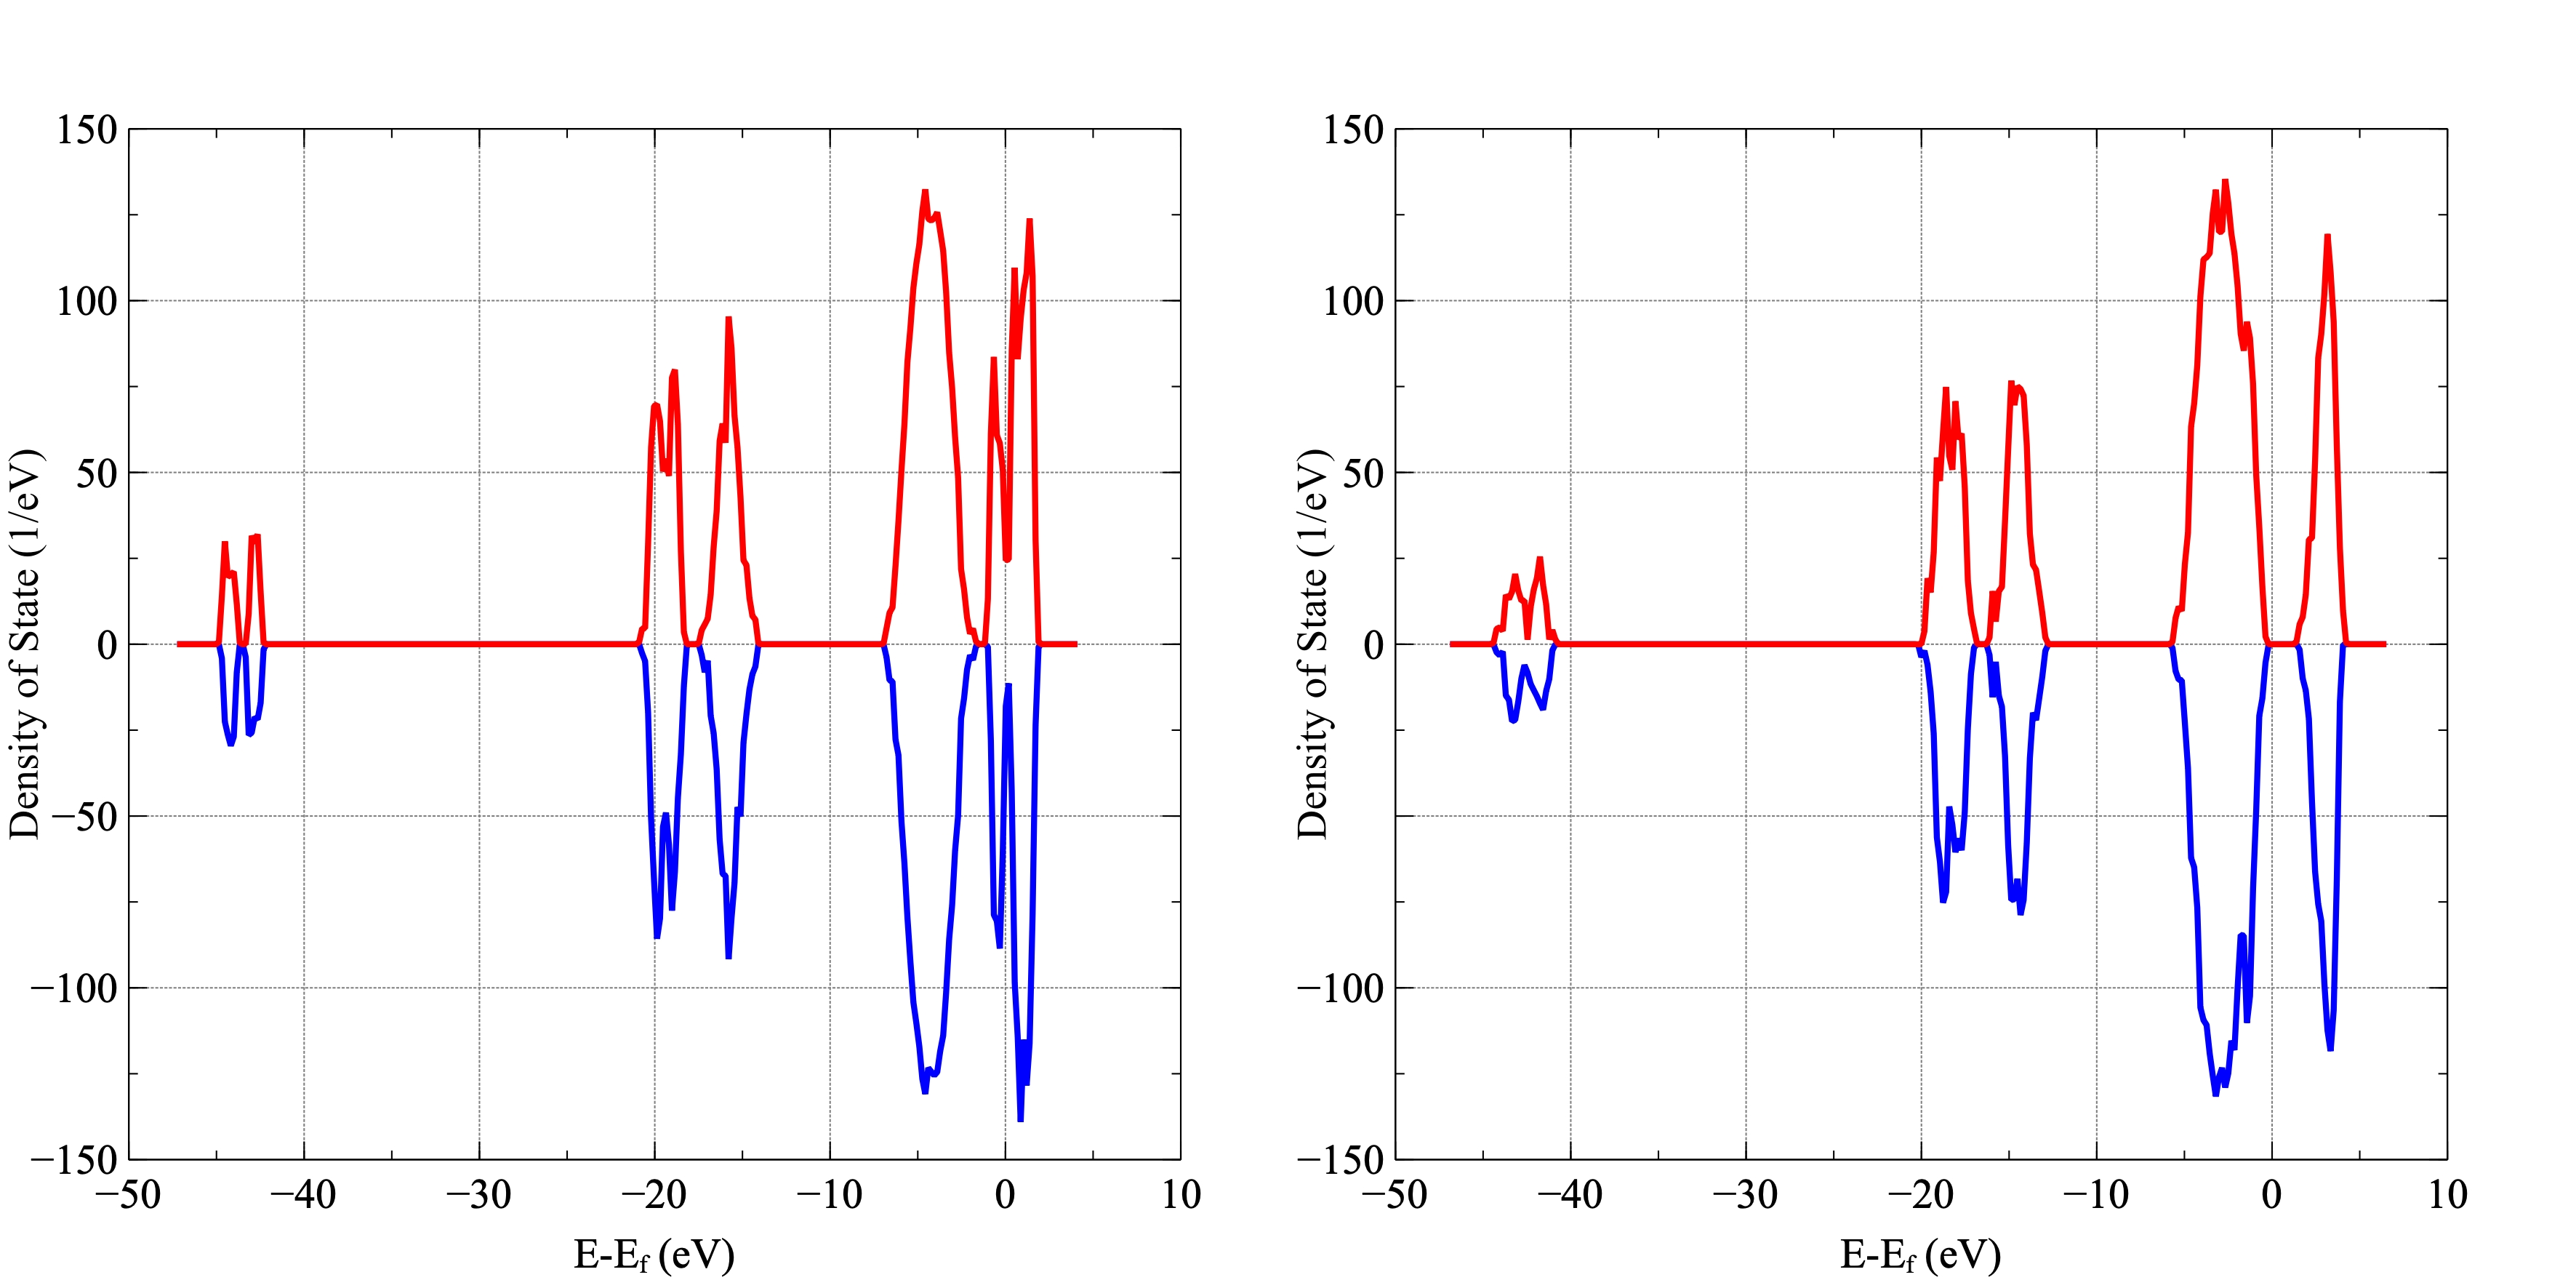
\includegraphics[width=0.9\textwidth]{fig3.jpg}
\caption{The predicted density of states for simulations of AFM molten UCl$_3$ at 1250 K, a) not including a Hubbard $U$ model, and b) a Hubbard U value of 4 eV. {\color{red}The density of states are ensemble averages of 200 steps.}}
\label{fig:DOS}
\end{figure*}


\subsection{AIMD simulations of NaCl}
\subsubsection{Density and structure}
Figure \ref{fig:NaCldensity}a plots the predicted density of molten NaCl as function of temperature for the DFT-D3, DFT-dDsC, and vdW-DF2 Van der Waals models as well as simulations without any dispersion interaction based strictly upon the Perdew-Burke-Ernzerhof (PBE) generalized gradient approximation \cite{pbe}. A correlation derived from experimental data is also shown~\cite{Janz1988}. The DFT-dDsC, DFT-D3, and PBE reproduce the temperature dependence of the density obtained from experiments. However, as expected, only the simulations that account for dispersion interactions are within 10\% of the experimental density correlation. The best agreement is obtained for the vdW-DF2 dispersion model, which is within 3\% or less of the experimental correlation across an extended temperature range. However, the DFT-dDsC dispersion model also correctly predicts the variation in density with temperature, whereas the vdW-DF2 underestimates the dependence. The calculated (DFT-dDsC and vdW-DF2) correlations for the density as function of temperature are listed in Table~\ref{table:NaCldensityetc}. The radial pair distribution function at 1250 K is reported in Figure \ref{fig:radial}b, which highlights first, second and third-shell coordination distances of 2.70~\AA, 3.78~\AA~and 4.14~\AA, respectively. The predicted pair distribution function is in good agreement with experimental values~\cite{Edwards_1975}. Further calculations did not include the DFT-D3 Van der Waals model or PBE without a Van der Waals description. 

\begin{figure*}[htb]
\centering
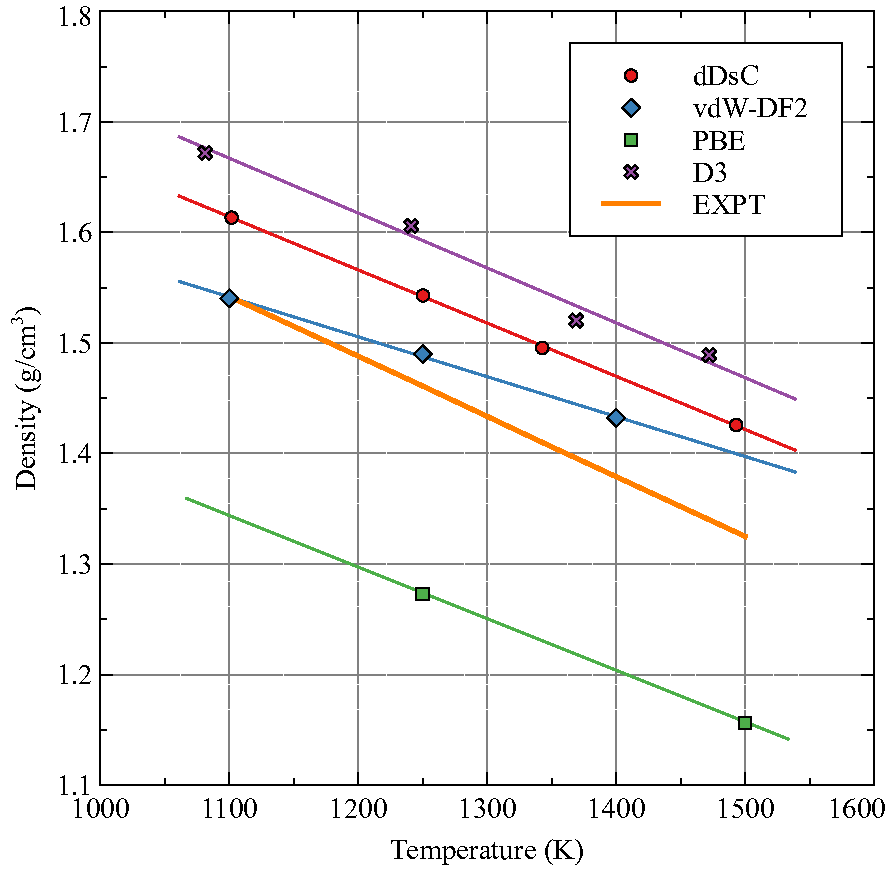
\includegraphics[width=0.6\textwidth]{fig4.pdf}
\caption{Density of NaCl predicted with two different models for dispersion forces (DFT-D3 and DFT-dDsC) and one without (small cell witih 64 atoms for DFT-dDsC, large cell with 208 atoms for others). Experimental data is represented by the correlation plotted as an orange line~\cite{Janz1988}.}  
\label{fig:NaCldensity}
\end{figure*}


\begin{table*}[hb!]
\centering
{\color{red} 
\begin{tabular}{lcc}
\hline
\hline
& Density (g/cm$^3$) &Heat capacity (J/mol/K) \\
\hline
NaCl Calculated (DFT-dDsC)	&$2.1438-0.0004814T$ ($1100 - 1500$ K) &69.0 ($1100 - 1500$ K)\\
NaCl Calculated (vdW-DF2)	& 1.9379-0.0003603T ($XX - YY$ K)& 58.1 ($XX - YY$ K)\\
NaCl Experiment	&$2.1381-0.0005426T$~\cite{Janz1988} ($1080-1300$ K) &66.9~\cite{NIST} \\	
UCl$_3$ Calculated (DFT-dDsC) &$5.9467-0.001257T$ ($1000-1500$ K) &141.4 ($1000-1500$ K)\\	
UCl$_3$ Calculated (vdW-DF2) &$4.7230-0.000554T$ ($XX - YY$ K) & 128.5 ($XX - YY$ K) \\	
UCl$_3$ Experiment	&$6.375-0.001522T$~\cite{Desyatnik} ($1138-1296$ K)&150~\cite{BENES2008},129.704~\cite{YIN2020} \\
\hline
\hline
\end{tabular}
}
\caption{Calculated and experimental correlations and values for density and heat capacity (C$_p$) of NaCl and UCl$_3$. {\color{red} Where known, the temperatures within parenthesis indicate the range of data used for fitting the models from either AIMD simulations or experiments.} }
\label{table:NaCldensityetc}
\end{table*}

\subsubsection{Heat capacity} 
The heat capacities are determined via Eq. \ref{eq:cp}, which is the slope of the total energy as a function of temperature. The constant pressure heat capacity (C$_p$) was obtained from the DFT-dDsC and the vdW-DF2 dispersion models, and is provided in Table \ref{table:NaCldensityetc} together with an experimental reference value~\cite{NIST}. The simulation results indicate a constant heat capacity {\color{red}(the total energy depends linearly on temperature within the accuracy of the simulation results)}, though in order to identify small deviations from this behavior a denser temperature mesh would be required. The good agreement between simulations and experiments for the heat capacity (see Table \ref{table:NaCldensityetc}) further emphasizes the accuracy of the AIMD simulations.

\FloatBarrier

\subsection{AIMD simulations of UCl$_3$}
\subsubsection{Density and structure}
Following the results for NaCl, the best performing Van der Waals models (DFT-dDsC and vdW-DF2) were applied to UCl$_3$. Figure \ref{fig:UCl3density}a) plots the predicted density for UCl$_3$ as function of temperature for the DFT-dDsC and vdW-DF2 dispersion models compared to three literature correlations derived from experiments~\cite{Janz1988,Desyatnik,Parker}. The Janz et al.~\cite{Janz1988} correlation for density is surprisingly different from the other two experimental references as well as from the present simulations. The temperature dependence is predicted to be close to linear across the full temperature range investigated. The DFT-dDsC simulations only slightly under-predict the density and temperature dependence compared to the experimental data due to Desyatnik et al.~\cite{Desyatnik} and Parker et al~\cite{Parker}. The vdW-DF2 results show a further under-prediction of the experimental densities from these two references, and a further reduction in the temperature dependence. The densities in Figure \ref{fig:UCl3density} were fitted to linear correlations and summarized in Table \ref{table:NaCldensityetc}. The simulations seem to confirm the validity of the experimental data due to Desyatnik et al.~\cite{Desyatnik} and Parker et al~\cite{Parker}, while the data from Janz et al.~\cite{Janz1988} is not supported.
 
The radial pair distribution function at 1250 K is reported in Figure \ref{fig:radial}a, which highlights a first-shell coordination distance of 2.82~\AA. The coordination distance is in excellent agreement with the experimental values of 2.82 \AA~\cite{Neilson} and 2.84 \AA~\cite{Okamoto} measured at 1113 K and 1200 K, respectively, while it is higher than the AIMD simulations by Li et al.~\cite{Li}, which can likely be ascribed to the application of the Hubbard $U$ methodology in the present study. The predicted U-Cl coordination number of about 7.5 at 1250 K is within the 6 to 8 range reported in experiments and previous simulations~\cite{Li,Neilson,Okamoto}. 

\begin{figure*}[htb]
\centering
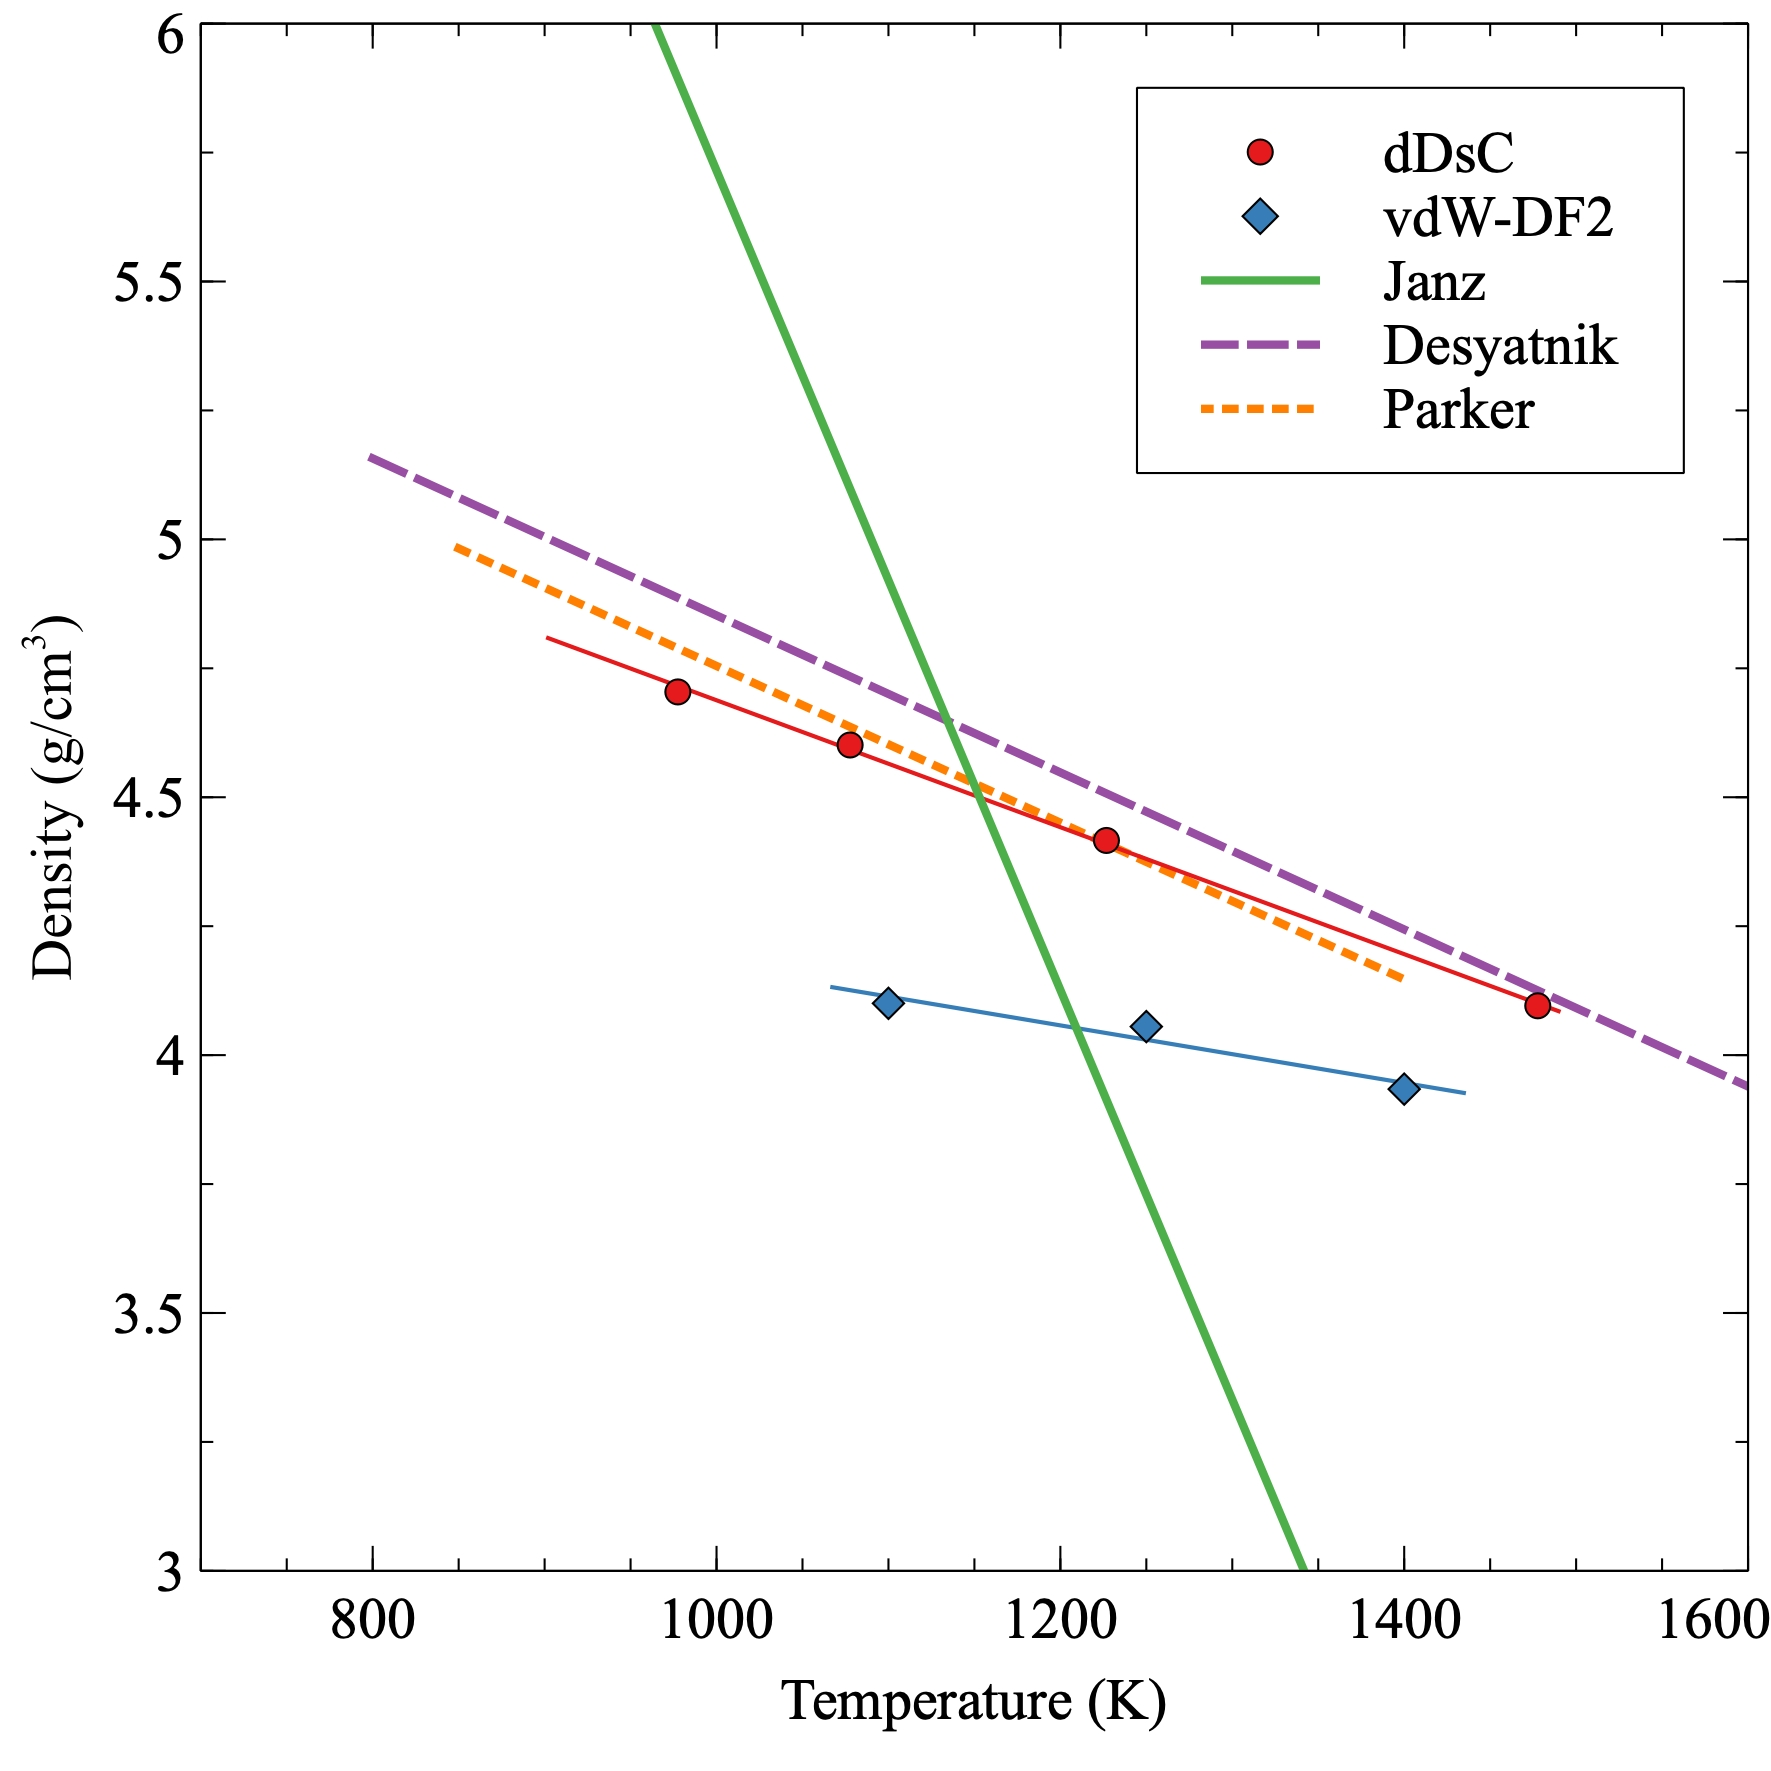
\includegraphics[width=0.6\textwidth]{fig5.jpg}
\caption{Density of UCl$_3$ predicted by the DFT-dDsC model for the dispersion forces (small cell with 64 atoms). Experimental data is represented by the correlations plotted as purple dashed~\cite{Desyatnik}, green solid~\cite{Janz1988} and orange dotted lines~\cite{Parker}. The lines following the calculated data points were obtained as least-squares fits, the equations of which are summarized in Table \ref{table:NaCldensityetc}.}  
\label{fig:UCl3density}
\end{figure*}

\subsubsection{Heat capacity} 
The heat capacities are determined as the slope of the total energy as a function of temperature. The total energy closely follows a linear relation as function of temperature and, consequently, the heat capacity can be approximated as a constant in the temperature range investigated. In order to resolve small deviations from the linear relation, a denser temperature mesh would have to be used. The constant pressure heat capacity (C$_p$) was obtained from the DFT-dDsC and the vdW-DF2 dispersion models and is provided in Table \ref{table:NaCldensityetc}. Experimental data for the heat capacity of UCl$_3$ has not been identified, but our DFT-dDsC value compares very well with the value derived from the Calphad assessment of the UCl$_3$ thermodynamics due to Benes et al.~\cite{BENES2008}, while it deviates somewhat from the assessment due to Yin et al.~\cite{YIN2020}. The comparison with the experimental data due to Benes et al.~\cite{BENES2008}  and Yin et al.~\cite{YIN2020} is reversed for the vdW-DF2 calculated heat capacity. 

\FloatBarrier

\subsection{Ab initio molecular dynamics simulations of NaCl-UCl$_3$}
\subsubsection{Density and structure}
The density of NaCl-UCl$_3$ mixtures were calculated for the DFT-dDsC and the vdW-DF2 dispersion models at three or four (depending on composition) different temperatures between 900 K and 1500 K, as shown in Figure \ref{fig:NaClUCl3}a. This figure also includes densities at the same temperatures as those of the simulations obtained from Redlich-Kister (RK) correlations \cite{agca2022} derived from experimental data due to Desyatnik et al.~\cite{Desyatnik} as well as data derived from the correlations reported by Parker et al.~\cite{Parker}. The simulated data points are generally within a few per cent of the experimental data, with slightly higher values in the UCl$_3$-rich region for the vdW-DF2 dispersion model.

\begin{figure*}[htb]
\centering
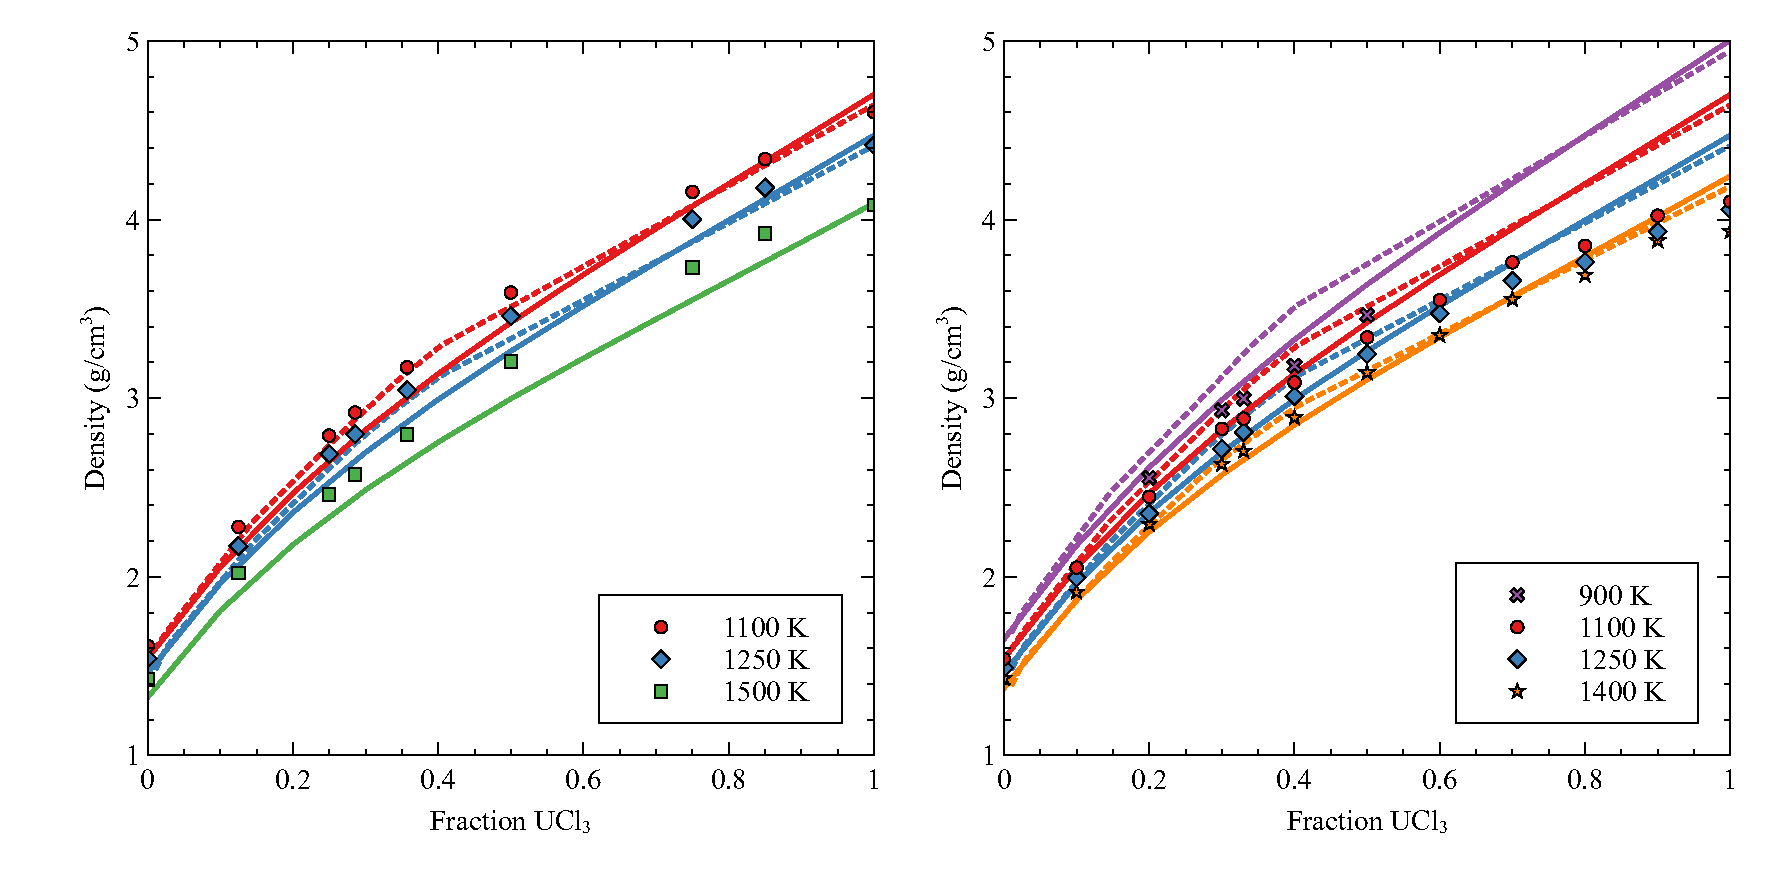
\includegraphics[width=0.9\textwidth]{fig6.pdf}
\caption{Density of NaCl-UCl$_3$ mixtures as obtained from simulations using the (a) DFT-dDsC dispersion formulation, and (b) the vdW-DF2 dispersion formulation at temperatures between 900 K and 1500 K. The solid lines represent the Redlich-Kister correlation to the Desyatnik \cite{Desyatnik} data from Agca \cite{agca2022}. The dotted lines are calcualted from experimental correlation due to Parker \cite{Parker}.} 
\label{fig:NaClUCl3}
\end{figure*}

The deviation from ideal mixing for the DFT-dDsC dispersion is shown in Figure \ref{fig:ideal} and compared to the experimental deviation from ideal mixing from Desyatnik \cite{Desyatnik} and data derived from the densities reported by Parker et al.~\cite{Parker}.  
It is challenging to converge the density for mixed salt solutions to an accuracy better than around one per cent of the absolute density using AIMD simulations, which gives rise to some scatter in the data points. Nevertheless, a few trends are discernible from Figure \ref{fig:ideal}. The simulations suggest a negative deviation from an ideal solution (lower density than predicted by an ideal solution behavior) by up to 2\%, except close to pure UCl$_3$ at high temperature where a positive deviation is observed. According to our simulations, the magnitude of the deviation from ideal solution behavior is a function of composition and varies with temperature starting at $x\approx0.35$ and continuing in the UCl$_3$-rich composition range, while it is almost independent of temperature in the NaCl-rich range. 
The maximum deviation from ideal solution behavior occurs close to the eutectic composition of 35\% UCl$_3$, perhaps slightly shifted towards the NaCl-rich side but it is hard to draw a solid conclusion due to uncertainties in the simulated data. These predictions are qualitatively similar to the correlations derived from experiments by Desyatnik et al.~\cite{Desyatnik}, though the experimental correlations predict a larger magnitude for the deviation from an ideal solution and also exhibit a stronger temperature dependence than the simulations. The data points for the deviation from ideal solution behavior due to Parker et al.~\cite{Parker} are scattered around the ideal solution trend line with a possible trend towards a positive deviation for the higher temperatures.
Compared to the simulations based on a polarizable ion model performed in Ref.~\cite{VANOUDENAREN2021117470} at 1100 K, the present AIMD simulations predict a consistent and slightly larger negative deviation from ideal solution behavior.

\begin{figure*}[htb]
\centering
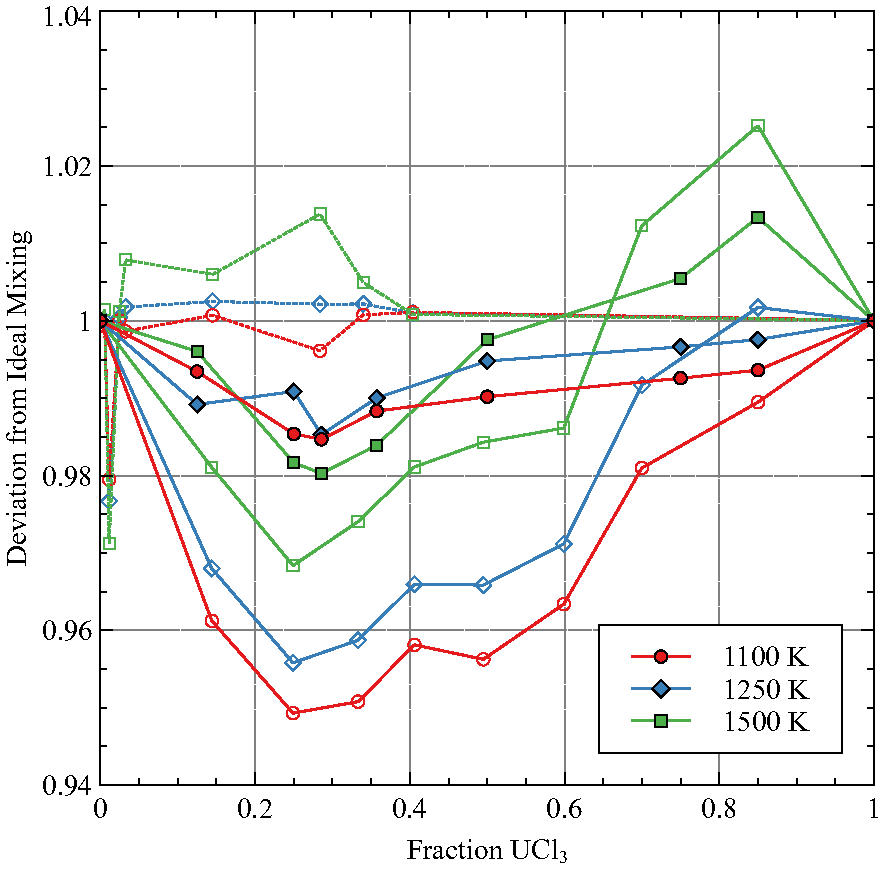
\includegraphics[width=0.6\textwidth]{fig7.pdf}
\caption{The fractional deviation form ideal solution behavior plotted as function of composition at temperatures between 1100 K and 1500 K. The solid symbols represent the simulation data and the open symbols represent the experimental data from Desyatnik \cite{Desyatnik}. The open symbols with the dotted lines represent points derived from the experimental correlations reported by Parker et al.\cite{Parker}.} 
\label{fig:ideal}
\end{figure*}

The density as a function of temperature displays a linear dependence for all compositions, with a unique slope at each given composition, similar to the pure end-members. The coefficients describing the linear dependence on temperature for each composition are plotted in Figure \ref{fig:TandCp}. Although there is some scatter, a weak non-linear dependence on composition for both the linear and constant term (not shown) is identified. The non-linear dependence is most pronounced in the UCl$_3$-rich range. The density behaviors identified in Figures \ref{fig:NaClUCl3}, \ref{fig:ideal}, and \ref{fig:TandCp} can also be expressed in a combined composition-temperature dependent correlation:
\begin{equation}
\begin{split}
\rho(x,T)=\frac{M_{NaCl}(1-x)+M_{UCl_3}x}{\frac{M_{NaCl}(1-x)}{\rho_{NaCl}}+\frac{M_{UCl3}x}{\rho_{UCl_3}}}+(e_1+e_2T)x(1-x)+(f_1+f_2T)x(1-x)(2x-1), 
\label{eq:LS}
\end{split}
\end{equation}

\noindent where the first term represents the density of an ideal solution and the subsequent terms the deviation from ideal solution behavior using a Redlich-Kister expansion. $M_{NaCl}$ and $M_{UCl_3}$ are the molar masses of the end-member salts, $\rho_{NaCl}$ and $\rho_{UCl_3}$ the temperature dependent densities of the end-member salts, which are taken from the correlations previously derived, $T$ is temperature and $x$ is the mole fraction of UCl$_3$ in the mixture. This is a similar formulation to the Redlich-Kister model from Agca \cite{agca2022}. A least-squares fit of the coefficients describing deviation from an ideal solution are collected in Table \ref{table:LS}. 
 The resulting fit captures the absolute densities well, but cannot reproduce all the features of the deviation from ideal solution behavior shown by the calculated data points in Figure \ref{fig:ideal}, which is a consequence of the sharp transition at x=0.30 and the stronger temperature dependence exhibited in the UCl$_3$-rich range for T = 1500 K compared to the lower temperatures. 

\begin{figure*}[htb]
\centering
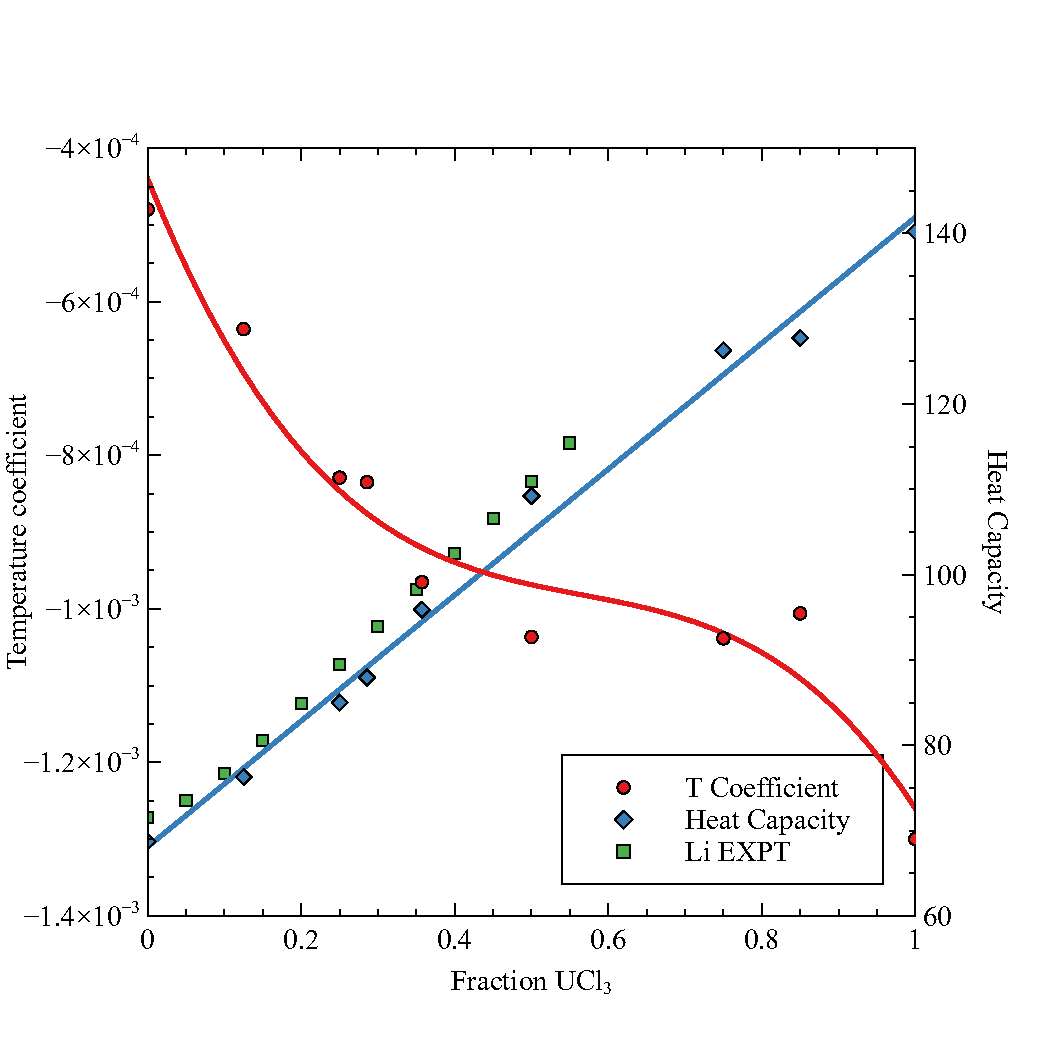
\includegraphics[width=0.6\textwidth]{fig8.pdf}
\caption{The coefficient describing the linear temperature dependence of density and the heat capacity as function of the UCl$_3$ fraction. The solid line for the temperature coefficient represents a least-squares fit of a third order polynomial. The solid line for the heat capacity represents a least-squares fit of a linear correlation. {\color{red}Data points calculated from the heat capacity relation derived by Li \textit{et al.} \cite{Li2020} from semi-empirical MD simulations are included for comparison, but only for the composition range where the relation was fitted (x(UCl$_3$)$<0.55$).}}
\label{fig:TandCp}
\end{figure*}

\begin{table}[hb!]
\centering
{\color{red}
\begin{tabular}{lcc}
\hline
\hline
&Density (Eq. \ref{eq:LS}) &Mixing energy (Eq. \ref{eq:LSE}) \\
\hline
$e_1$ &-0.37928 (g/cm$^3$) &-0.29088 (eV) \\
$e_2$ &0.00021185 (g/cm$^3$/K) &0 (eV/K)\\
$f_1$ &-1.1043 (g/cm$^3$) &0.058987 (eV) \\
$f_2$ &0.0010322 (g/cm$^3$/K) &0 (eV/K)\\
\hline
\hline
\end{tabular}
}
\caption{A least-squares fit of the coefficients describing density and mixing energy of the NaCl-UCl$_3$ system as function of temperature, see Eqs. \ref{eq:LS} and \ref{eq:LSE}.}
\label{table:LS}
\end{table}

\FloatBarrier

\subsubsection{Heat capacity and mixing energy}
The total energy for each NaCl-UCl$_3$ composition displays a linear dependence as a function of temperature, similar to the pure NaCl and UCl$_3$ systems. The heat capacity for each composition can be obtained from the slope of the total energy versus temperature, and this heat capacity is displayed in Figure \ref{fig:TandCp}. The heat capacity displays a monotonic increase with composition that exhibits an ideal mixing type behavior. Thus, for a given composition of the pseudo-binary salt, a linear interpolation of the heat capacities is an appropriate approximation. {\color{red}Data points calculated from the heat capacity relation as function of UCl$_3$ composition derived by Li \textit{et al.} \cite{Li2020} from semi-empirical MD simulations are included for comparison, but only for the composition range where the relation was fitted (x(UCl$_3$)$<0.55$). The agreement between the two simulation data sets is very good.}

The mixing energies of NaCl-UCl$_3$ at temperatures ranging from 1100 K to 1500 K as calculated by the DFT-dDsC dispersion formulation are plotted in Figure \ref{fig:mixing}, with the NaCl and UCl$_3$ end-members as reference points. The mixtures exhibit a negative deviation from ideal solution behavior, which implies that the solution phase is favored over a two-phase mixture of the end-points. 
 The minimum (most negative) mixing energy is between $x$=0.35 and $x$=0.5, which qualitatively mimics the results for the density, perhaps with a slight shift towards the 50-50 composition. 
  
 The mixing energy was measured at 1100 K by Matsuura et al.~\cite{Matsuura} and the results are also shown in Figure \ref{fig:mixing}. They indicate very good agreement with the simulations across the full composition range. In addition to the experimental data points, there are two sets of thermodynamic models for the mixing energy~\cite{BENES2008,YIN2020}, and the correlation from Ref.~\cite{YIN2020} is included in Figure \ref{fig:mixing}. Both thermodynamic models assume the mixing energy to be independent of temperature, which is in good agreement with the simulations. The model by Yin et al.~\cite{YIN2020} was derived from the experimental measurements by Matsuura et al.~\cite{Matsuura} and consequently agree similarly well with our simulation results. The model by Benes et al.~\cite{BENES2008} exhibits a smaller mixing energy than both the experimental data points and our simulations, but is not shown in Figure \ref{fig:mixing}. 

\begin{figure*}[htb]
\centering
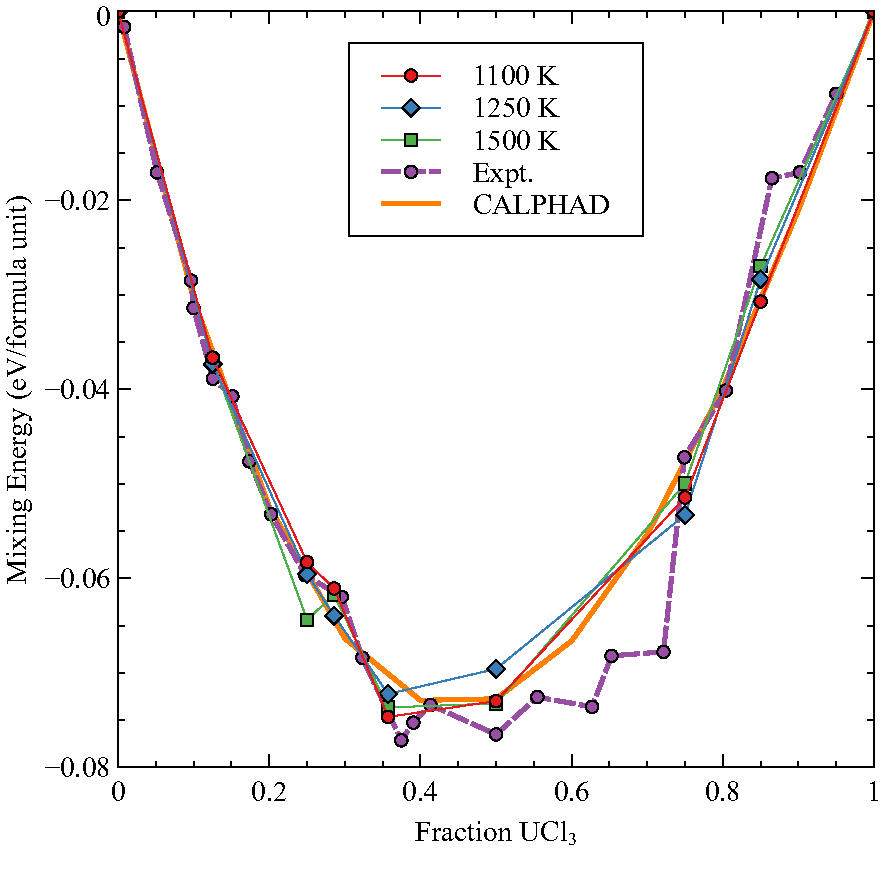
\includegraphics[width=0.6\textwidth]{fig9.pdf}
\caption{Mixing energies for NaCl-UCl$_3$ at 1100, 1250 and 1500 K. Pure NaCl and UCl$_3$ are used as references. The calculated results are compared to experiments~\cite{Matsuura} and a thermodynamic assessment~\cite{YIN2020}.} 
\label{fig:mixing}
\end{figure*}

Based on the AIMD results, the following expression may be fitted to the mixing energy as function of composition and temperature:
\begin{equation}
\begin{split}
E_{mix}(x,T)=(e_1+e_2T)x(1-x)+(f_1+f_2T)x(1-x)(2x-1),
\label{eq:LSE}
\end{split}
\end{equation}
where the parameters for all the temperature-dependent terms are set to zero based on the lack of discernible temperature dependence in Figure \ref{fig:mixing}. This expression is equivalent to the Redlich-Kister expansion used in existing Calphad models. The coefficients resulting from the fit to the data in Figure \ref{fig:mixing} are summarized in Table \ref{table:LS}. Heat capacity may be derived as the derivative of Eq. \ref{eq:LSE}, but would be equal to zero due to the lack of temperature dependence. The heat capacity of mixtures are given by a linear interpolation of the end-members, see Figure \ref{fig:TandCp}.

\FloatBarrier

\subsubsection{Compressibility}

The degree of compressibility of a fluid has strong implications for its dynamics. The compressibility is determined as the negative of the derivate of the volume as a function of pressure, divided by the volume at a given pressure, as in Eq. \ref{eq:compress}. The pressure at a series of volumes was identified and a second-order polynomial was fit to the dependence. This second-order polynomial served as the base function to obtain the derivative of the volume with respect to pressure. The volume of interest is identified as that at which the pressure is zero for a given temperature and composition. The temperature and composition-dependent compressibility is displayed in Figure \ref{fig:compress}. Given the isothermal nature of the simulations, this data can be considered to be isothermal compressibility. There is a decrease in the compressibility both with increasing UCl$_3$ fraction and with decreasing temperature. The magnitudes indicate a liquid that is more compressible than water at room temperature and atmospheric pressure (46$\times$10$^{-11}$ Pa$^{-1}$), less compressible than mercury (3.7 $\times$10$^{-11}$ Pa$^{-1}$), and comparable to glycerin (21$\times$10$^{-11}$ Pa$^{-1}$) \cite{aiphandbook}. As can be observed in Eq. \ref{eq:compress}, the compressibility is the reciprocal of the bulk modulus, and can thus be interpreted in the inverse manner. As such, UCl$_3$ has a higher bulk modulus than NaCl. Additionally, the bulk modulus softens with increasing temperature, as would be expected. 

\begin{figure}[htb]
\centering
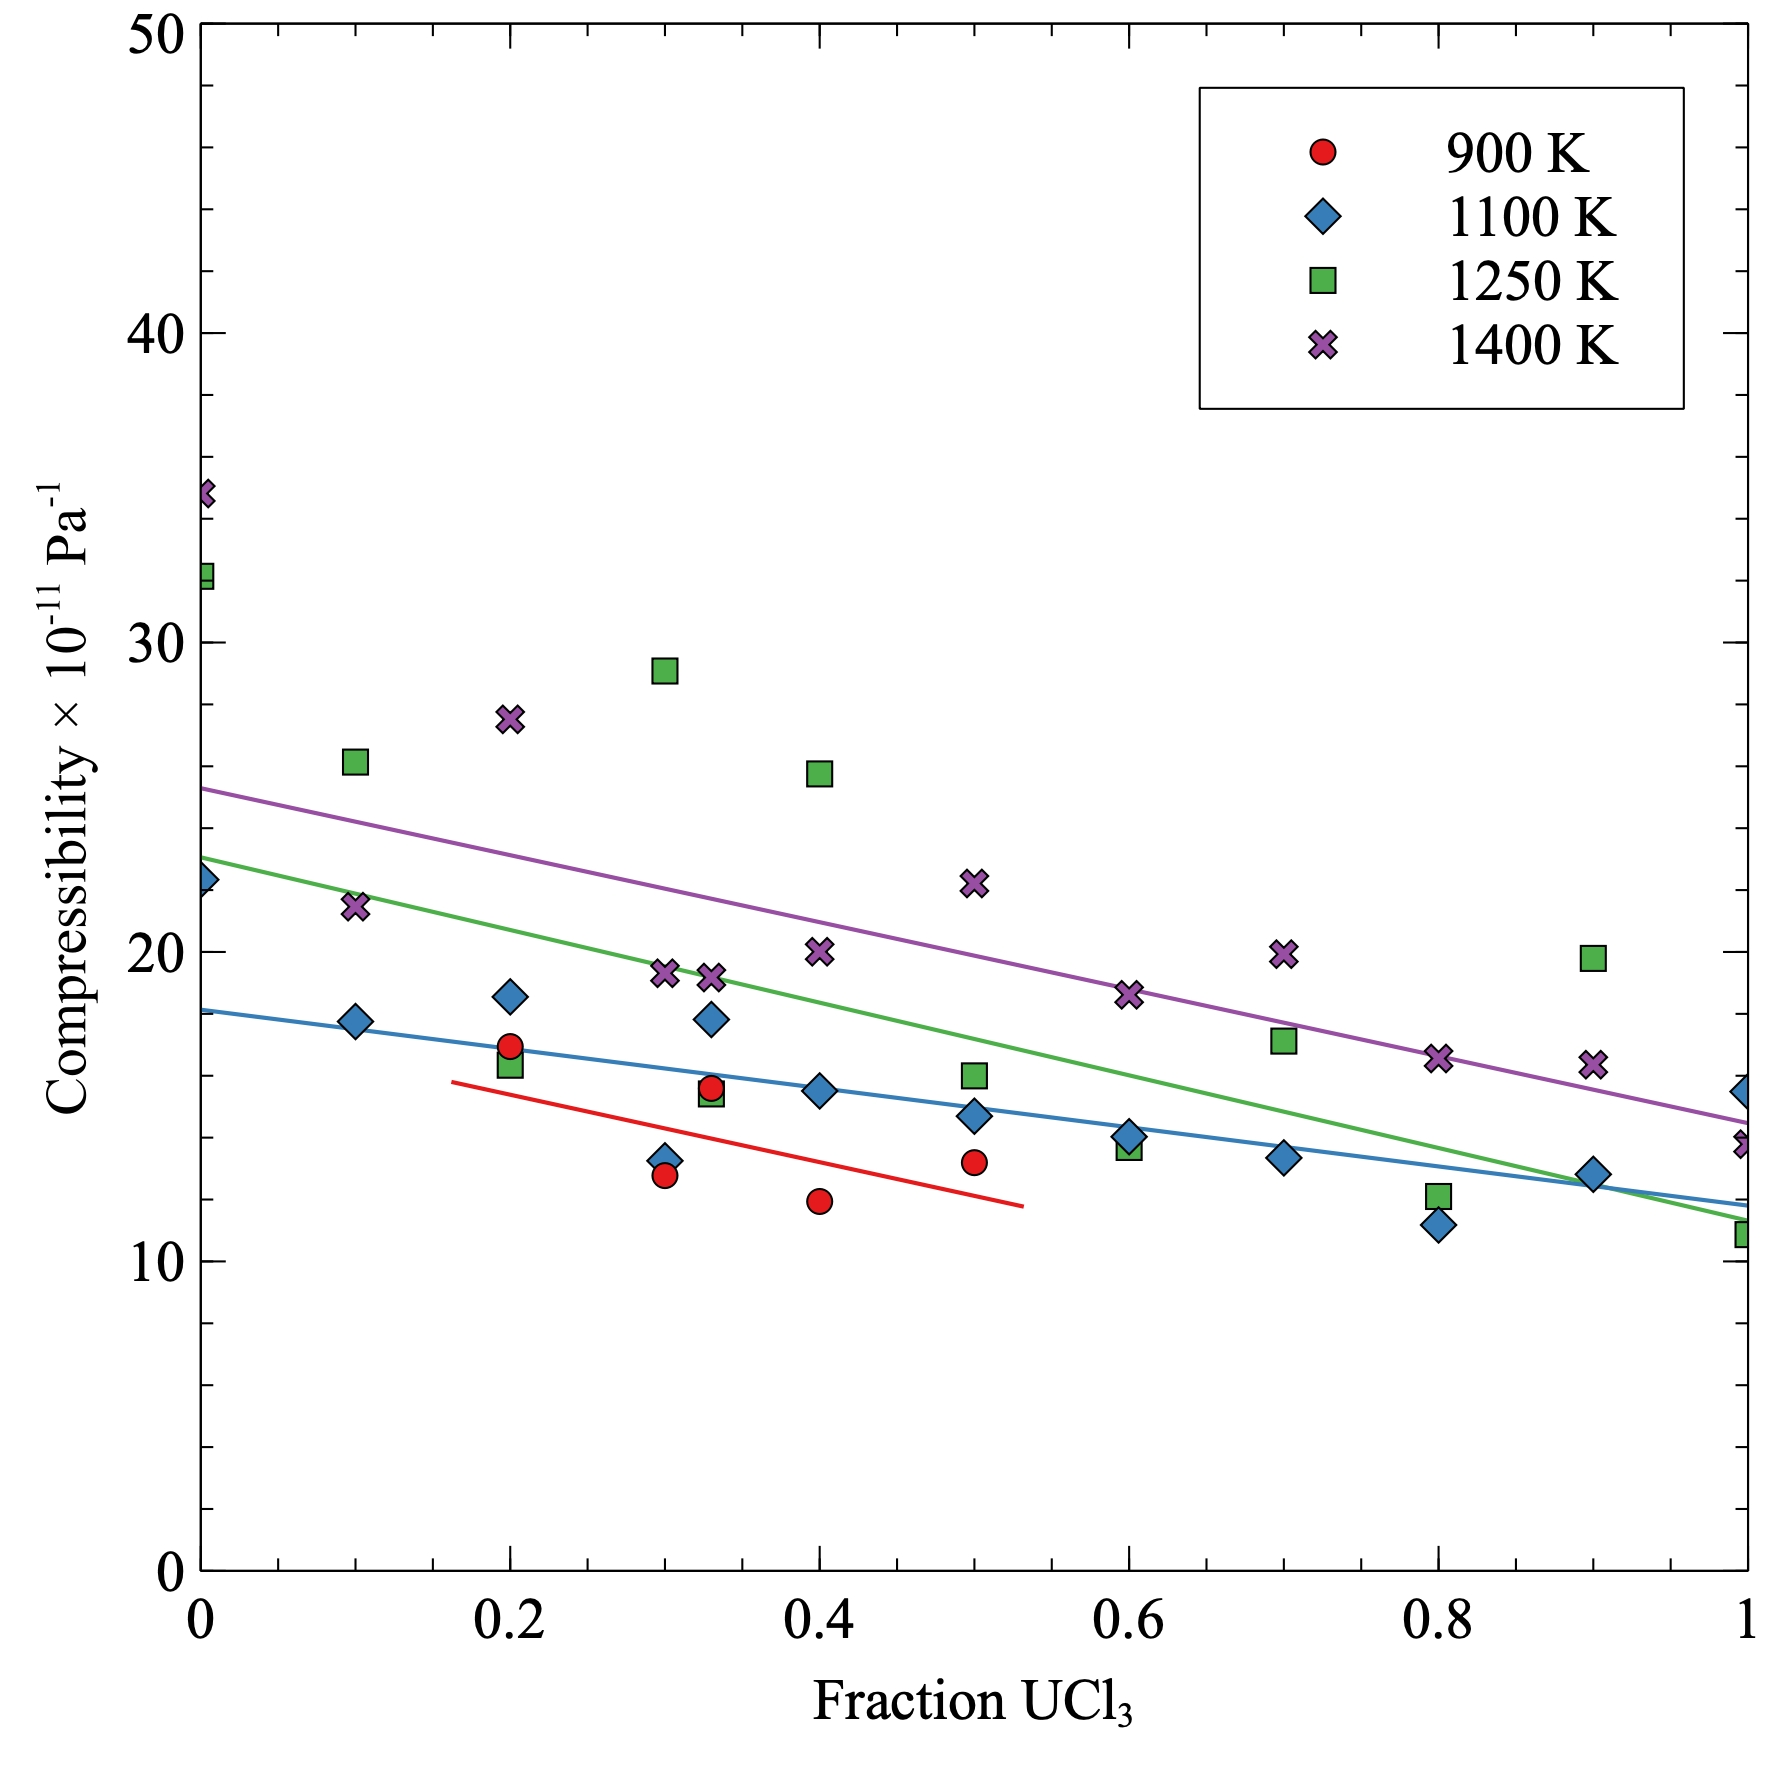
\includegraphics[width=0.6\textwidth]{fig10.jpg}
\caption{Calculated compressibilities for the NaCl-UCl{$_3$} pseudo-binary as a function of composition at four temperatures. Linear fits to the data are included to better illustrate trends in the data and do not imply a linear relationship.} 
\label{fig:compress}
\end{figure}

\FloatBarrier

\subsubsection{Diffusivity}
The diffusion coefficients for each individual species, as well as the total diffusion coefficient, are plotted as a function of composition and temperature in Figure \ref{fig:diff}. The diffusion coefficients follow a similar trend as function of temperature for all compositions in that D$_{Na}$ $>$ D$_{Cl}$ $>$ D$_U$. Additionally, the diffusion coefficients decrease with increasing UCl$_3$ content. However, the most rapid diffusion is found for the pure UCl$_3$ system. Arrhenius fits to the data can be applied, as in Figure \ref{fig:arrhenius}, and tabulated in Table \ref{table:diff}. The migration energies as calculated from the Arrhenius fits show a near monotonic increase with increasing UCl$_3$ content. The increase in the diffusion coefficient for pure UCl$_3$ is due to the larger pre-factor. The results for NaCl compare favorably with previous experimental measurements of diffusivities. While this work predicts a Na diffusion coefficient in NaCl of 4.7$\times$10$^{-9}$ m$^2$/s, experimental measurements have determined a value of 8.0 $\times$10$^{-9}$ m$^2$/s \cite{janz_diffusion}. Additionally, Na diffusion proceeding more rapidly in NaCl than Cl diffusion has been observed experimentally \cite{janz_diffusion}. No experimental diffusion data has been obtained for the pure UCl$_3$ or the NaCl-UCl$_3$ system. \color{red}{In the absence of such experimental data, comparisons must be made to existing computational studies. While there are no AIMD investigations into diffusion in the NaCl-UCl$_3$ system, two prior studies utilizing classical molecular dynamics with a polarizable ion model interatomic potential (Li) \cite{Li} and a machine learning interatomic potential (Nguyen) \cite{nguyen_ML} have studied diffusion in the NaCl-UCl$_3$ system. While neither of these studies included the composition and temperature ranges explored within this work, there are general comparisons that can be made. Li showed the same relative diffusion pattern (D$_{Na}$ $>$ D$_{Cl}$ $>$ D$_U$), while Nguyen predicted Cl diffusion to proceed more quickly than Na diffusion. Li provided diffusion as a function of temperature at two compositions (5 mol\% and 50 mol\% UCl$_3$), showing that diffusion decreases and the activation energy increases with increasing UCl$_3$ content, in agreement with this work. However, Li did not provide pre-factors or units in their Arrhenius plots, making direct comparisons difficult. However, all of the qualitative trends in this work are consistent with that of Li. Nguyen only studied the eutectic composition, and only at temperatures below 1100 K. Comparing the data at their maximum temperature (1070 K) and our minimum temperature (1100 K), all of the diffusion coefficients, including individual species and total diffusion, are within a factor of four, indicating excellent agreement. Additionally, Nguyen determined the activation energy of the eutectic composition to be 0.39 eV, which is similar to our calculation of 0.3 eV. While the qualitative trends in species diffusion differ between this work and that of Nguyen, the quantitative values generally agree quite well.  }

\begin{figure}[htb]
\centering
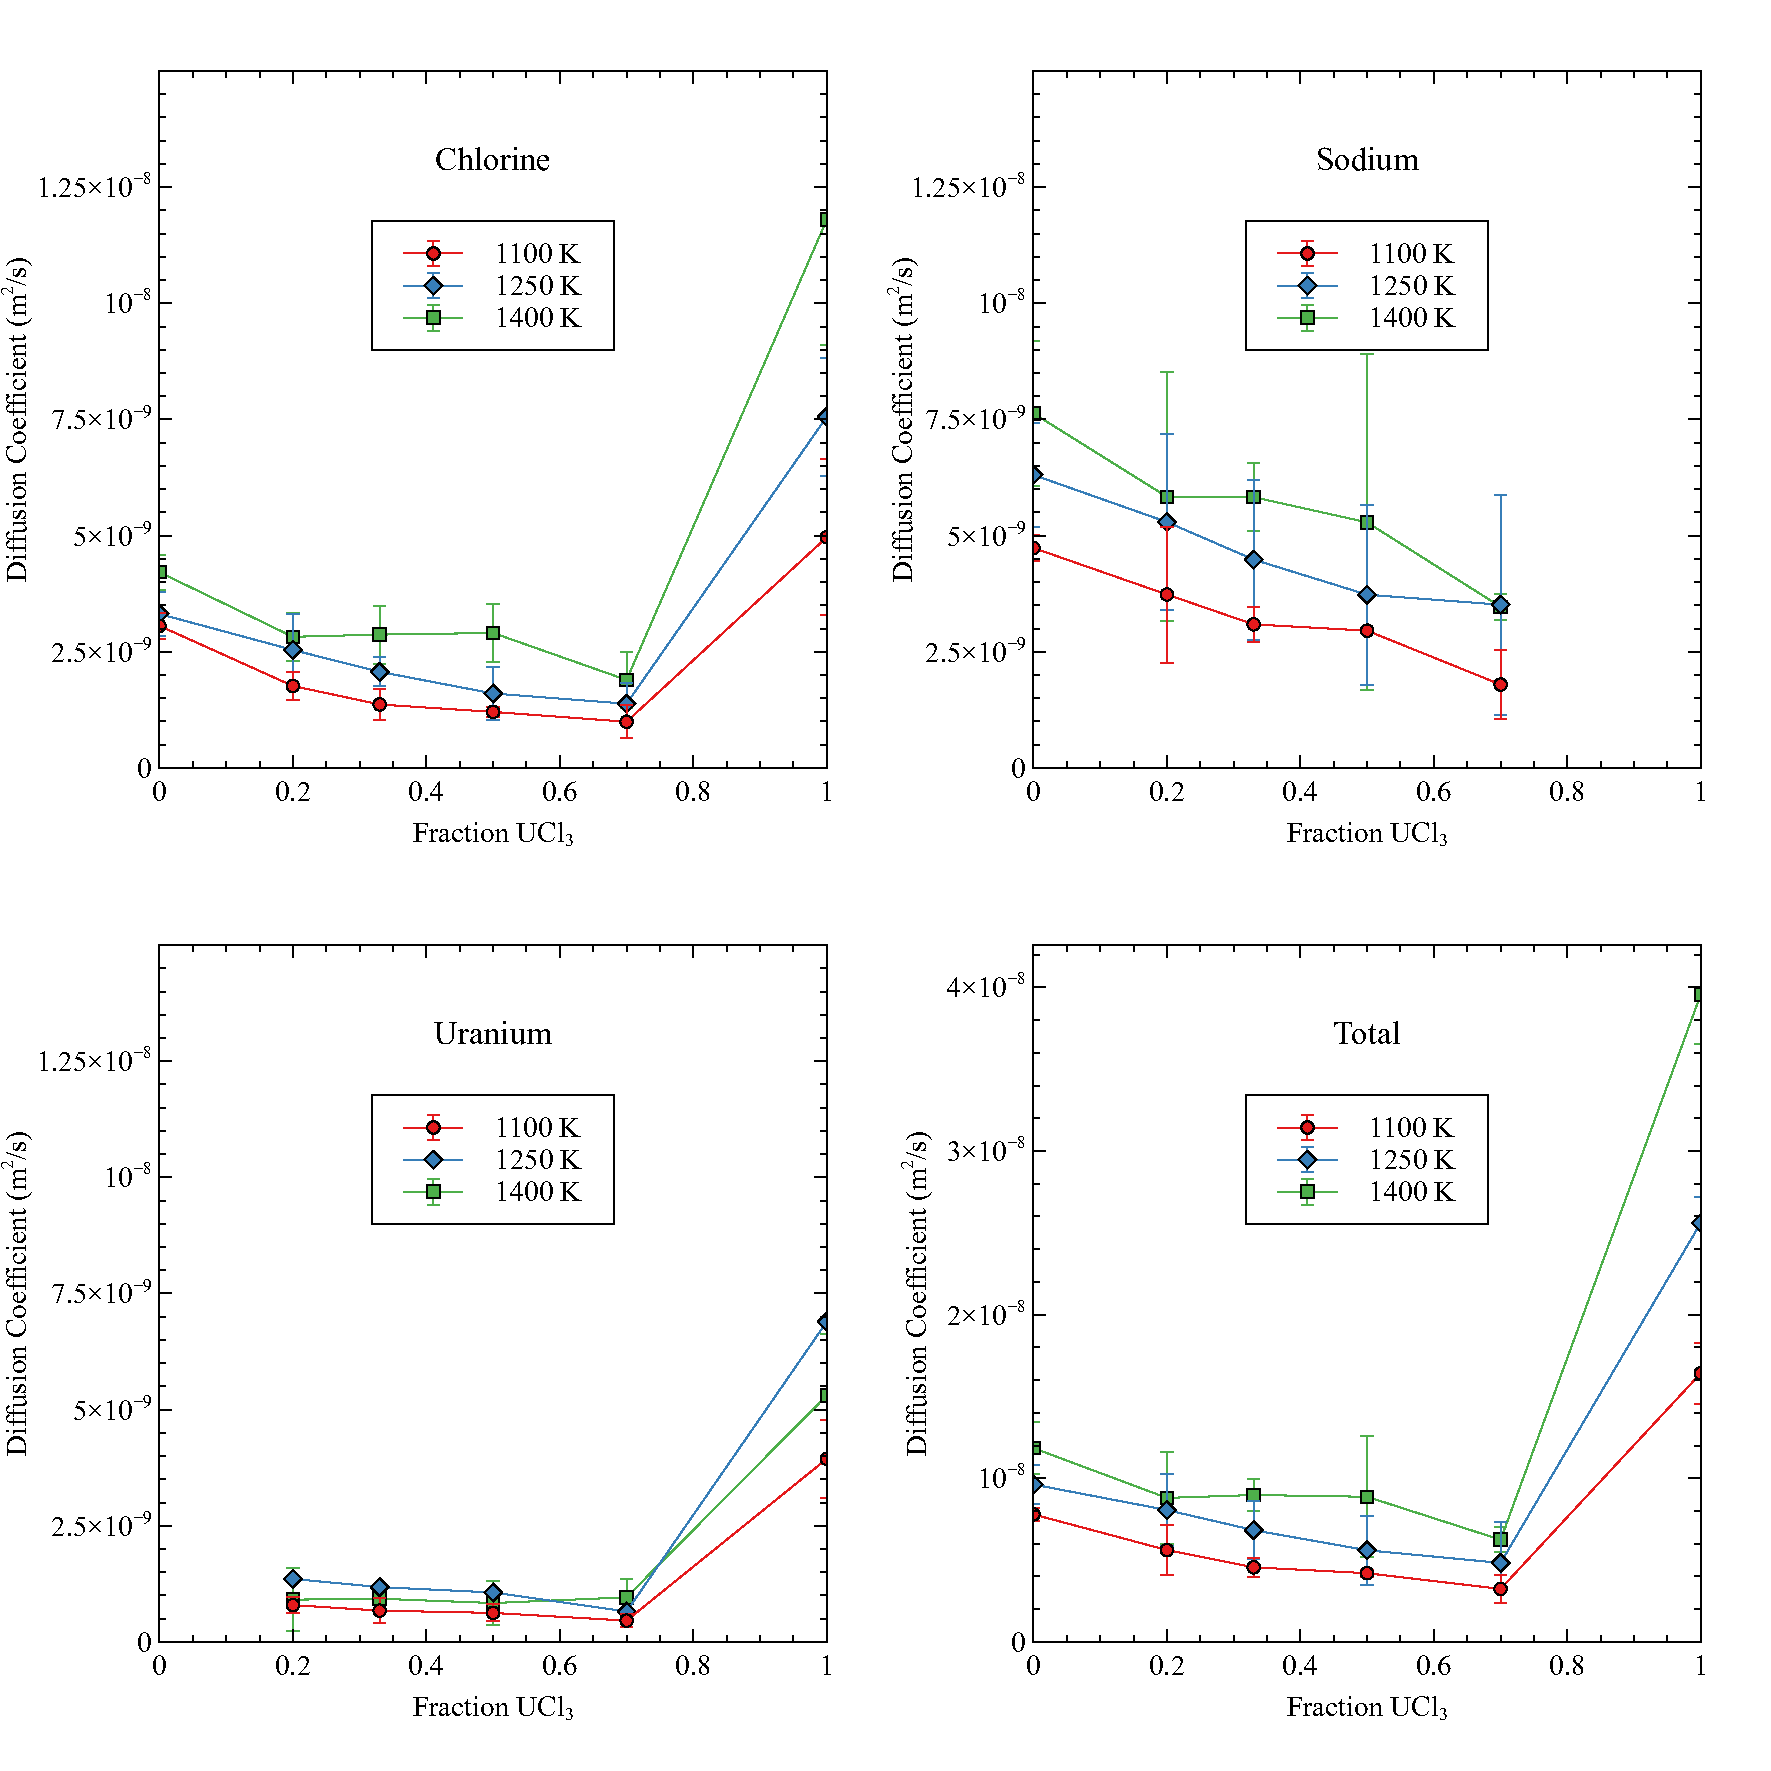
\includegraphics[width=0.9\textwidth]{fig11.pdf}
\caption{Calculated diffusivities for each species in NaCl-UCl{$_3$} and the total diffusivity as function of temperature. \color{red}{The error bars represent twice the standard error of the mean.} } 
\label{fig:diff}
\end{figure}

\begin{figure}[htb]
\centering
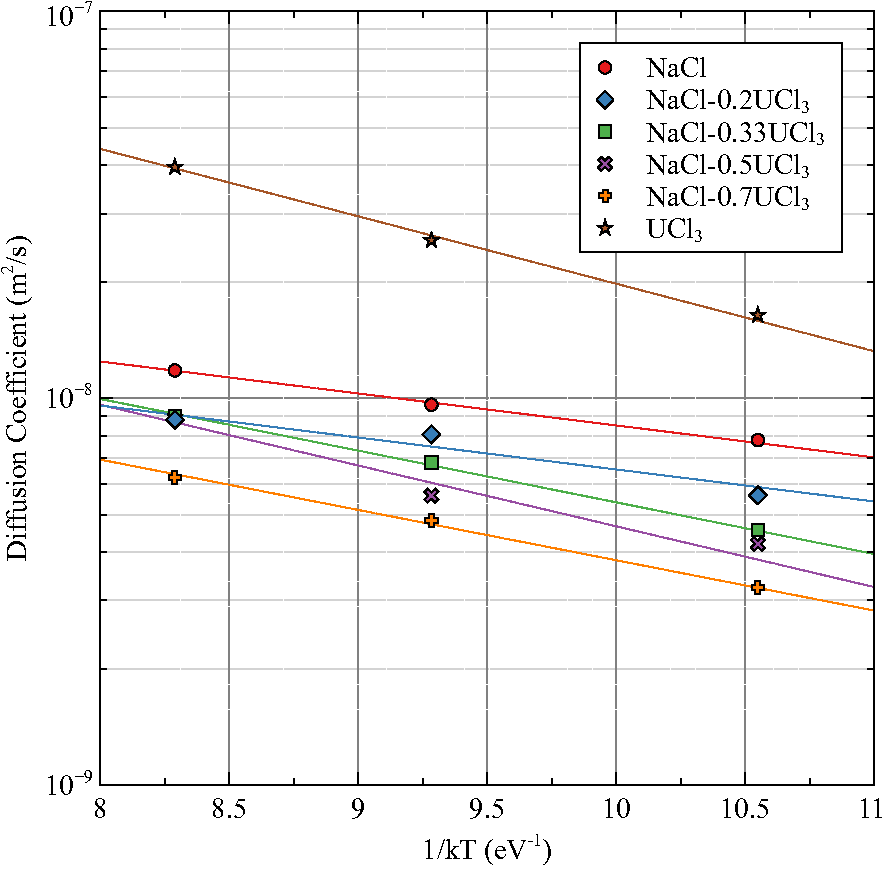
\includegraphics[width=0.6\textwidth]{fig12.pdf}
\caption{Arrhenius diffusion in NaCl-UCl{$_3$} \color{red}{at six unique compositions from 1100 K - 1400 K.}} 
\label{fig:arrhenius}
\end{figure}

\begin{table*}[hb!]
\centering
\caption{Prefactor and migration energy for the total diffusion in NaCl-UCl$_3$ systems\color{red}{, where D = D$_0${\times}exp(-E$_m$/(k$_b$T)).}}
\begin{tabular}{lccc|}
\hline
\hline
Fraction UCl$_3$	&	D$_0$(m$^2$/s)	&	E$_m$(eV)	\\
\hline
0	&	5.41E-08	&	0.184	\\
0.2	&	4.93E-08	&	0.203	\\
0.33	&	1.10E-08	&	0.301	\\
0.5	&	1.26E-07	&	0.326	\\
0.7	&	7.10E-08	&	0.292	\\
1	&	9.65E-07	&	0.388	\\
\hline
\hline
\end{tabular}
\label{table:diff}
\end{table*}


\FloatBarrier

\section{Discussion}
\label{sec:discussion}
This discussion section is focused on the behavior of mixed salts, in particular how the mixing properties (energy and density) relate to the evolution of the pair distribution functions and coordination numbers in the mixed salts. Figure \ref{fig:fig_pair} plots the pair distribution functions at four salt compositions ($x=0.25$, $x=0.29$, $x=0.36$ and $x=0.50$) at 1250 K and compares them to the reference pair distribution functions for UCl$_3$, while Figure \ref{fig:fig_coord} shows the U-Cl and U-U coordination numbers as function of the UCl$_3$ composition. The trends to be discussed below are the same for the other compositions and temperatures that were investigated (T=1100 K and T=1500 K).
 
Ref.~\cite{Li} identified networks of UCl$_3$ units above a fractional UCl$_3$ concentration of 0.30, and more isolated units below this concentration. This behavior is also visible in the pair distribution functions (see Figures \ref{fig:fig_pair}). The U-U pair distribution function for mixtures with a composition equal to or above a fractional UCl$_3$ concentration of 0.5 maintain the same or very similar shape and height as in pure UCl$_3$, which emphasizes the importance of UCl$_3$ network formation in the mixtures. Only the x(UCl$_3$)=0.5 case is shown in Figure \ref{fig:fig_pair}, but the U-U pair distribution function for x(UCl$_3$)=0.75 and x(UCl$_3$)=0.87 overlap with that of the pure system. Somewhere between x(UCl$_3$)=0.5 and x(UCl$_3$)=0.36, the U-U pair distribution function starts to deviate from that in pure UCl$_3$, which indicates that the network structure is starting to break up or change. This behavior is visible in the third coordination shell in Figure \ref{fig:fig_pair}. 
Below a fractional concentration of 0.36, in particular for x(UCl$_3$)=0.29 (Figure \ref{fig:fig_pair}b), the U-U pair distribution function further deviates from the pure UCl$_3$ case, revealing an inability to maintain the favorable network structure. 
Related changes may be observed in other distribution functions. Figure \ref{fig:fig_pair}a seems to indicate a closer resemblance to the U-U coordination in UCl$_3$ for x(UCl$_3$)=0.25 than for x(UCl$_3$)=0.29. This is believed to be a consequence of partial phase separation in the salt, where the U ions organize to fulfill the coordination at the most favorable composition between x(UCl$_3$)=0.36 and x(UCl$_3$)=0.50. The remaining NaCl units exist in separate domains. {\color{red}However, it is important to acknowledge that the small size of the simulation cells limits the ability to draw strong conclusions. More expansive simulations would be required for that purpose, which is beyond the scope of the present study.} 
Figure \ref{fig:fig_coord} shows that the U-U coordination number gradually decreases with the NaCl concentration, as expected. The data points follow a weak quadratic relation, with the samples that are unable to maintaining the U-U pair distribution function deviating slightly from that trend (x(UCl$_3$)=0.125, x(UCl$_3$)=0.30 and x(UCl$_3$)=0.36).
The limited size of the simulation supercells and somewhat limited sampling in the time domain imply that it can be challenging to recover the ideal ionic coordination in the UCl$_3$-poor region. Small variations in the ionic coordination noticeably impact the energy and volume. For example, it is possible that the x(UCl$_3$)=0.29 and x(UCl$_3$)=0.36 cases in Figures \ref{fig:fig_pair}b and c can reach a U-U pair distribution that is slightly closer to the pure UCl$_3$ case if the simulations were either run for a longer time or utilized a larger supercell. In that case, the predicted energy in Figure \ref{fig:mixing} would be expected to be slightly lower. The modified coordination would impact the predicted densities as well. Despite these simulation challenges, the results presented in this study are believed to closely represent the minimum energy solution at the temperature of interest and capture the preferred coordination, but it is important to acknowledge that the complex coordination chemistry creates simulation challenges with associated uncertainty. For constant pressure simulations the supercell may distort significantly to optimize the coordination chemistry.

The location of the transition from a network structure governed by the U-U coordination in UCl$_3$ to a partial network structure or partial phase separation, approximately coincides with the minimum in the mixing energy and the maximum deviation of the density from an ideal solution (compare Figures \ref{fig:NaClUCl3}, \ref{fig:mixing} and \ref{fig:fig_pair}), even though the latter may be skewed to a slightly lower UCl$_3$ content. In turn, these coincide with the eutectic composition according to the experimental phase diagram~\cite{YIN2020}. Combined with the U-U pair distribution function in the mixtures, this suggests that the negative mixing energy is driven by incorporating the NaCl units within the UCl$_3$ network, 
but if the fractional UCl$_3$ concentration is below $\approx0.36$, the gain from incorporating the NaCl units is countered by not being able to maintain the favorable U-U coordination seen in UCl$_3$, as evidenced by the break-up of the network structure or partial phase separation. The balance of incorporating the  NaCl units and maintaining UCl$_3$ network is posited to be responsible for the minimum in the mixing energy and by extension the location of the eutectic point in the phase diagram. The possible existence of a partial phase separation below the preferred mixing composition ($\approx 0.36$) is further emphasized by the mixing energy in Figure \ref{fig:mixing} approximately following a straight line from x(UCl$_3$)= 0.36 to x(UCl$_3$)= 0, which suggests that the behavior is governed by the two end-points. Additional work is required to ascertain these observations, but that is beyond the scope of the present study.

 \begin{figure*}[htb]
\centering
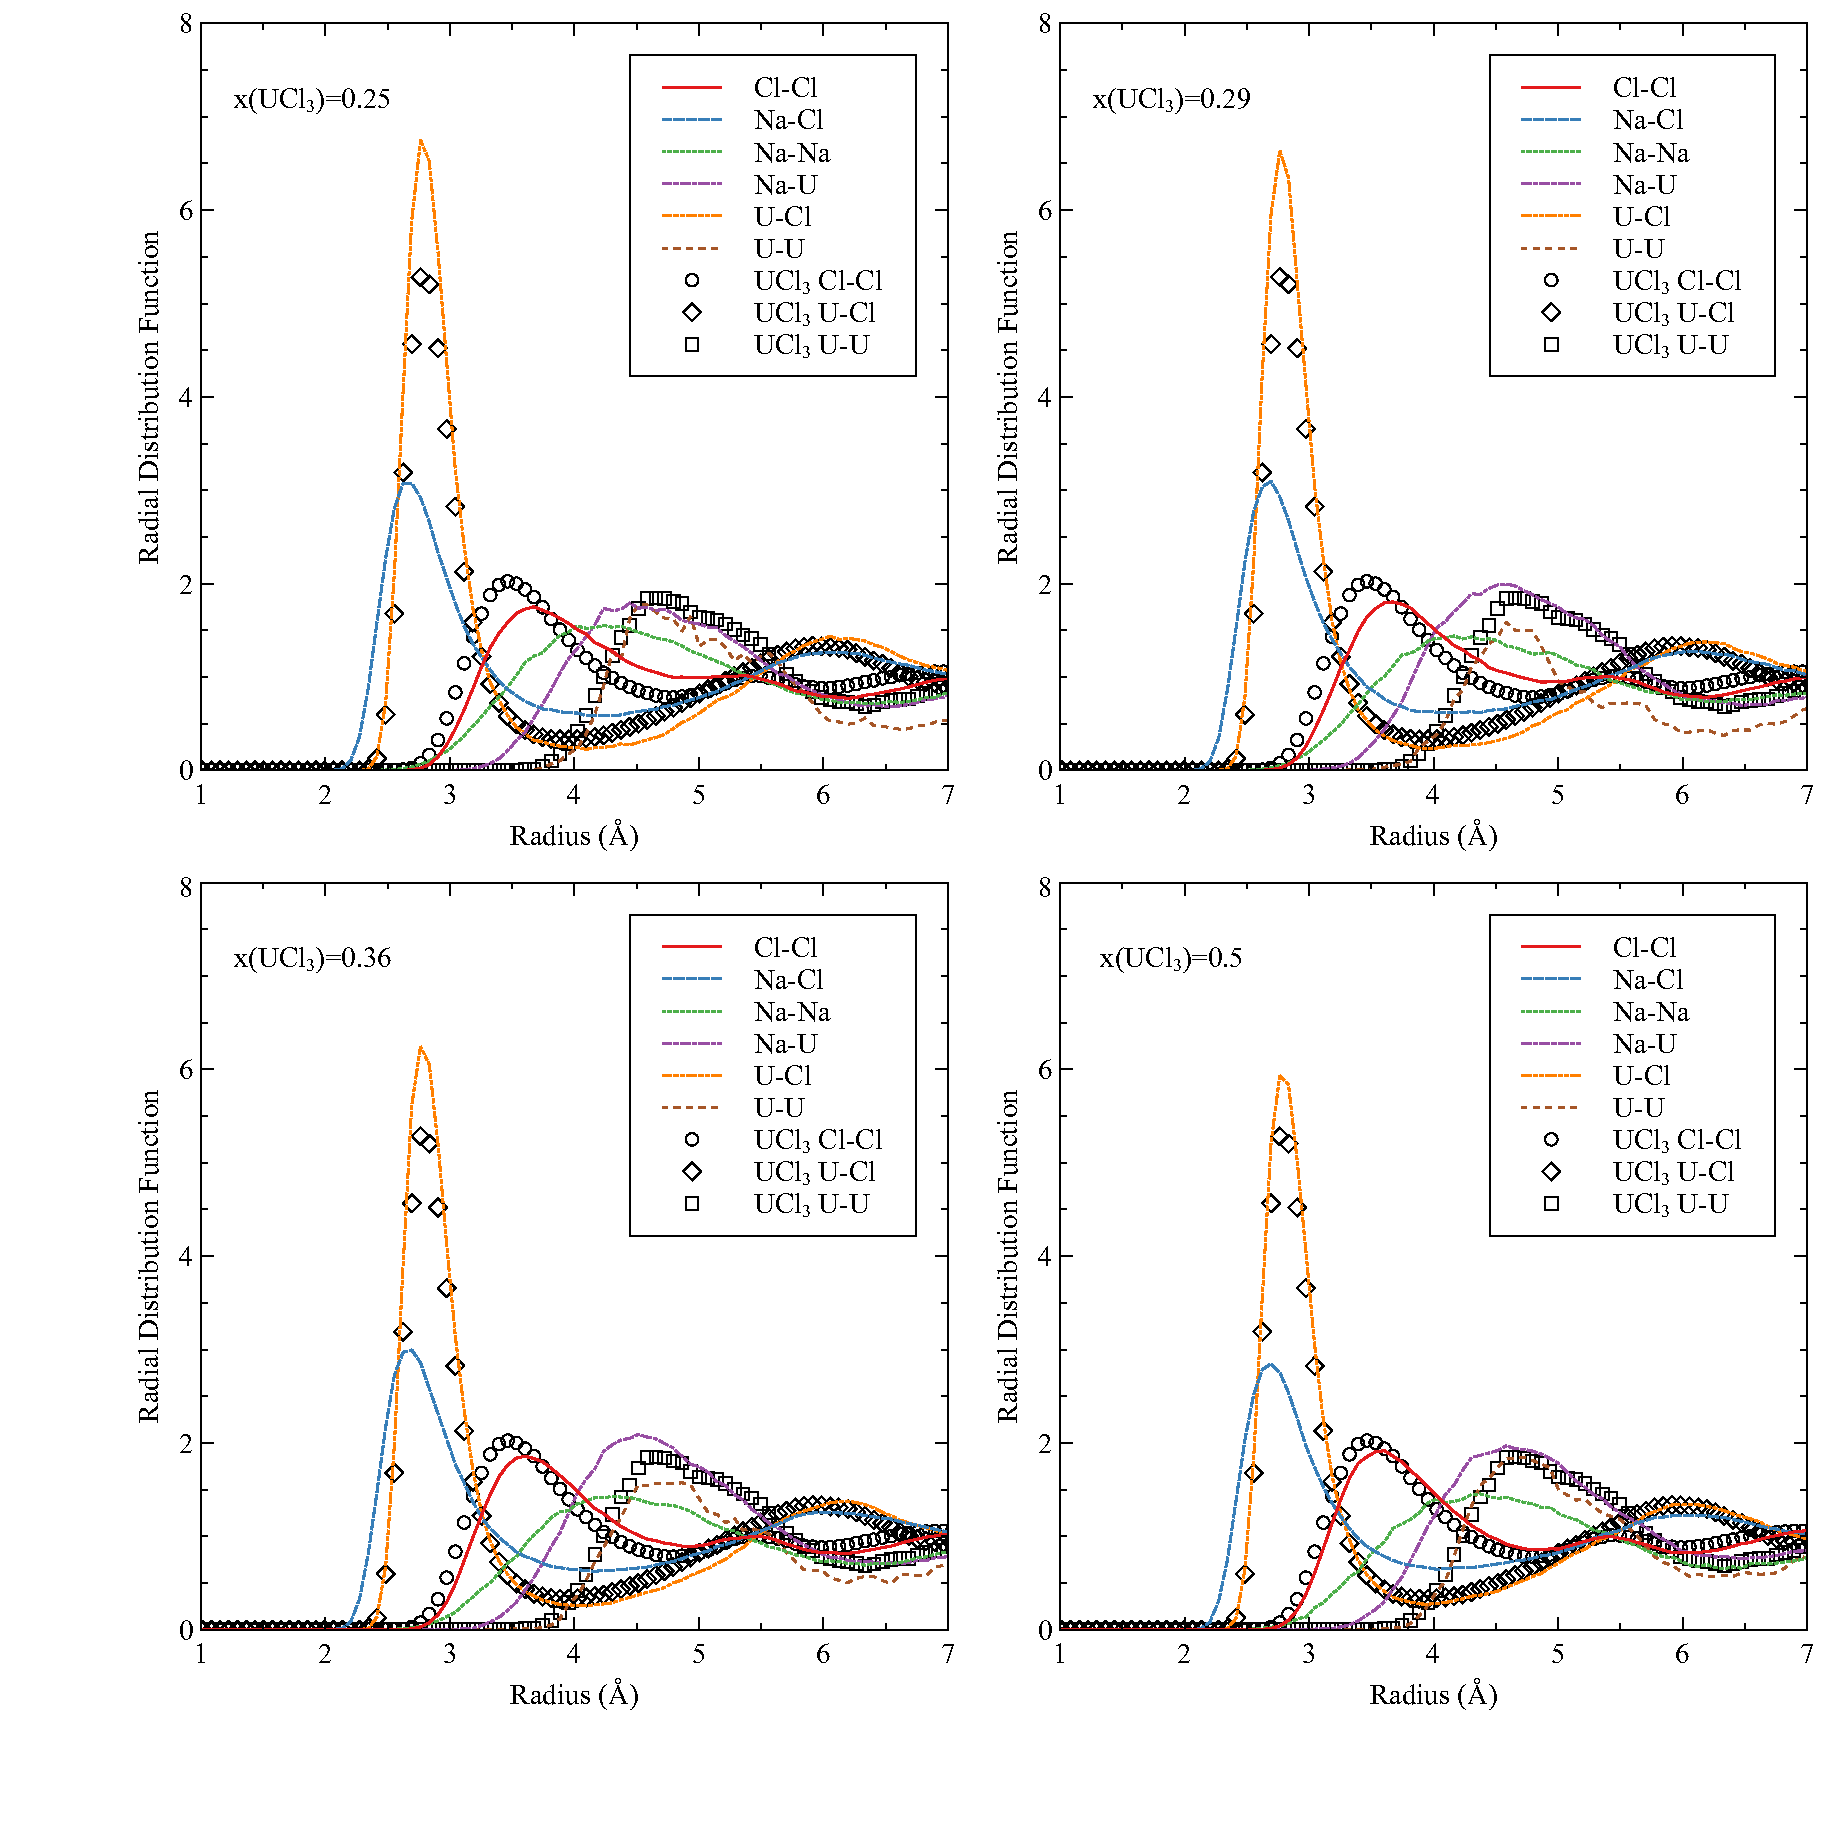
\includegraphics[width=0.95\textwidth]{fig13.pdf}
\caption{Pair distribution functions for NaCl-UCl$_3$ mixtures as function of composition ($x=0.25$, $x=0.29$, $x=0.36$ and $x=0.50$). The reference U-Cl and U-U pair distribution functions for UCl$_3$ are plotted in each figure for comparison.} 
\label{fig:fig_pair}
\end{figure*}


 \begin{figure}[htb]
\centering
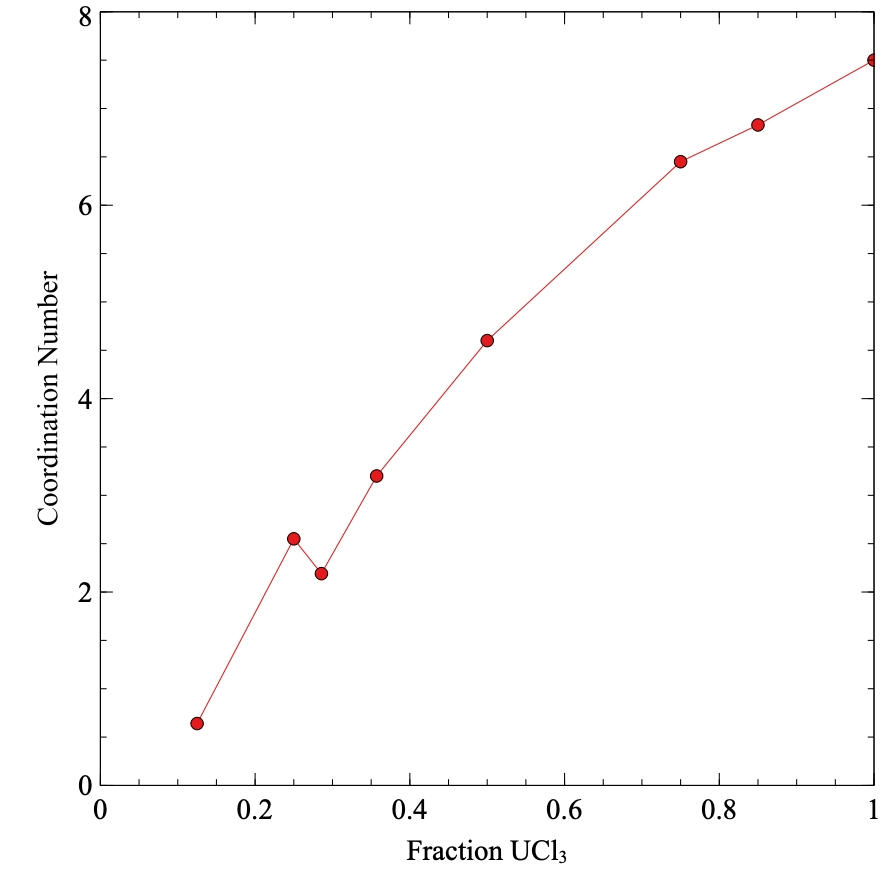
\includegraphics[width=0.6\textwidth]{fig14.jpg}
\caption{U-U coordination number as function UCl$_3$ content at T=1250 K.} 
\label{fig:fig_coord}
\end{figure}



\FloatBarrier

\section{Summary and conclusions}
\label{sec:conclusions}
Development of next-generation molten salt reactors (MSRs) require accurate thermodynamic and thermophysical properties of fuel-bearing salt mixtures and how those change with composition as well as with the addition of corrosion and fission products. The challenges associated with handling radioactive and corrosive salts make experimental measurements difficult. Using atomic scale simulations to fill these data gaps and to provide mechanistic understanding of property relations would facilitate more accurate evaluation of various concepts by reactor designers, developers, and other interested parties. Modeling and simulation have an important role to play in reducing data gaps, because the compositional space of interest is extensive and difficult to cover with experiments alone, especially since some of the salts are also highly toxic or radioactive. 

Following this recipe, AIMD simulations relying on different models for Van der Waals interactions were used to predict temperature-dependent thermophysical (density, thermal expansion, compressibility, and diffusion) and thermodynamic (mixing energy and heat capacity) properties of NaCl mixed with UCl$_3$. AIMD simulations of the pure end-member systems are able to accurately reproduce experimental data on densities and heat capacities provided that Van der Waals interactions are included in the simulations. 
Mixtures of UCl$_3$ with NaCl exhibit a negative mixing energy, with a minimum between $x=0.36$ and $x=0.50$, which is close to the eutectic composition. 
For NaCl-UCl$_3$, the mixing energy is predicted to be independent of temperature. The predicted mixing energy for NaCl-UCl$_3$ agrees very well with available experimental data. 
The existence of a minimum for mixing energy is related to the evolution of the radial distribution function and the tendency of UCl$_3$ to form network structures.
For a UCl$_3$ fraction less than approximately 0.36, the U-U network is unable to be fully maintained and the U-U pair distribution function deviates from that in pure UCl$_3$, which leads to a smaller mixing energy (less favorable). The $x=0.36$ composition approximately coincides with the observed eutectic composition. Below $x=0.36$ there seems to be a tendency to partially phase separate into regions mimicking the most preferred coordination and NaCl-rich regions. Related to the mixing energies, the heat capacity is predicted to be a linear function of composition in the mixed salts.

The same interactions that control the mixing energy also govern the evolution of the density for mixed salts. NaCl-UCl$_3$ exhibits a maximum deviation from ideal solution behavior at $x=0.30$. The densities of the mixed salts are lower than for the ideal mixture. The maximum deviation is about 2\% for NaCl-UCl$_3$ and is only weakly dependent on temperature, but the deviation from ideal solution behavior exhibits some temperature dependence in the UCl$_3$-rich range. 
 The predicted densities for the mixed systems agree at least qualitatively with available experimental data and the predictions are bound by data from the various experimental sources. 

The compressibility was calculated for the NaCl-UCl$_3$ system and there is a decrease with increasing UCl$_3$ fraction and with decreasing temperature. The magnitudes indicate a liquid that is more compressible than water at room temperature and atmospheric pressure, less compressible than mercury, and comparable to glycerin. UCl$_3$ is predicted to have a higher bulk modulus than NaCl. Additionally, the bulk modulus softens with increasing temperature, as would be expected. 

Finally, the diffusion coefficients were calculated and predicted to follow a similar trend for all compositions and temperatures in that $D_{Na} > D_{Cl} > D_{U}$. Additionally, the diffusion coefficients decrease with increasing UCl$_3$ content. However, due to a high pre-exponential factor, the most rapid diffusion is found for the pure UCl$_3$ system. Experimental diffusion data is only available for the NaCl system, for which the simulations are in good agreement. 

\section*{Acknowledgements}
This work was funded by the U.S. Department of Energy (DOE), Office of Nuclear Energy, Nuclear Energy Advanced Modeling and Simulation (NEAMS) program, the Los Alamos National Laboratory Directed Research and Development (LDRD) program, and the INL Laboratory Directed Research and Development (LDRD) Program. Los Alamos National Laboratory, an affirmative action/equal opportunity employer, is operated by Triad National Security LLC, for the National Nuclear Security Administration of the U.S.\ Department of Energy under Contract No. 89233218CNA000001. Idaho National Laboratory is operated by Battelle Energy Alliance, LLC with the U.S. Department of Energy under Contract No. DE-AC07-05ID14517. This research made use of the resources of the High-Performance Computing Center at Idaho National Laboratory, which is supported by the Office of Nuclear Energy of the U.S. Department of Energy and the Nuclear Science User Facilities.       


\bibliographystyle{elsarticle-num} 
\bibliography{Yellowjacket.bib}

\end{document}

